\documentclass[journal,compsoc]{IEEEtran}

\usepackage{amsmath,amssymb,amsfonts}
\usepackage{algorithmic}
\usepackage{algorithm}
\usepackage{array}
\usepackage{booktabs}
\usepackage{cite}
\usepackage{graphicx}
\usepackage{textcomp}
\usepackage{xcolor}
\usepackage{url}
\usepackage{multirow}
\usepackage[colorlinks=true, linkcolor=blue, citecolor=blue, urlcolor=blue]{hyperref}

\graphicspath{{./}{figures/}{../figures/}}

\begin{document}

\title{A Hybrid Dung Beetle Optimization and Marine Predators Algorithm (HDBO-MPA) for Trust-Aware Multi-Objective Service Discovery in Social IoT}

\author{Antigravity~Research~Consortium,~\IEEEmembership{Senior~Member,~IEEE}%
\thanks{Manuscript revised October 2026. Blinded for peer review. The authors are with the Center for Networked Intelligence and Pervasive Systems, Department of Computer Science and Engineering (correspondence e-mail: contact@antigravity-research.org).}%
}

\markboth{IEEE Internet of Things Journal,~Vol.~XX, No.~XX,~October~2026}%
{Antigravity Research Consortium: HDBO-MPA for Trust-Aware Service Discovery in Social IoT}

\maketitle

\begin{abstract}
Service discovery in the Social Internet of Things (SIoT) encounters severe operational vulnerabilities stemming from conflicting service quality criteria, battery depletion, and coordinated adversarial reputation attacks. Existing discovery techniques commonly rely on fixed scalar objective weighting~\cite{dahan2024innovative, singh2022trust} or encounter path infeasibility as a methodological challenge during continuous-to-discrete graph mapping. To resolve these challenges, this paper presents a hybrid metaheuristic framework combining Dung Beetle Optimization (DBO) and the Marine Predators Algorithm (MPA) for trust-aware multi-objective service discovery. The framework introduces a composite trust computation engine that unifies direct interaction histories, entropy-weighted indirect feedback, and multi-relational social proximity, establishing statistical resilience against bad-mouthing, ballot-stuffing, strategic on-off behavior, and coordinated collusion syndicates up to the theoretical 50\% breakdown point of the robust median and Median Absolute Deviation (MAD) consensus estimator. Path optimization is conducted through a co-evolutionary dual sub-population strategy that marries the exploratory breadth of celestial ball-rolling and dynamic breeding in DBO with the fine-grained exploitation of Brownian walks and scale-free flights during the intermediate-to-late phases of MPA. Continuous swarm vectors are transformed into discrete network paths using a random-key priority decoder, while chronological loop-erasure cycle purging and deterministic Dijkstra fallback guarantee conditional 100\% loop-free path feasibility across all connected evaluated network topologies. Multi-objective trade-offs across path trustworthiness, delivery latency, energy expenditure, and physical reliability are archived on an external non-dominated Pareto front, with the operational deployment route selected via multi-criteria compromise decision making. Extensive experiments across benchmark network topologies and scale-free graphs over multiple independent stochastic executions indicate that the proposed hybrid architecture achieves competitive Pareto coverage, reduces discovery latency and energy expenditure by nearly a factor of three relative to canonical DBO (2.8$\times$ and 3.2$\times$, respectively) and by approximately twofold relative to MPA (2.0$\times$ and 2.3$\times$, respectively), and maintains dependable service delivery under aggressive multi-vector attacks.
\end{abstract}

\begin{IEEEkeywords}
Social Internet of Things (SIoT), Service Discovery, Multi-Objective Optimization, Dung Beetle Optimization (DBO), Marine Predators Algorithm (MPA), Composite Trust Management, Collusion Attack Mitigation, Pareto Frontier, Multi-Criteria Decision Making (MCDM).
\end{IEEEkeywords}

\section{Introduction}
\IEEEPARstart{T}{he} Social Internet of Things (SIoT) paradigm transforms autonomous smart devices into socially connected entities capable of establishing friendship, co-location, co-work, and parental object relationships to facilitate distributed collaboration and contextual service discovery~\cite{marche2020how, rad2020social}. In massive smart-city and industrial deployments, resource-constrained edge devices frequently lack autonomous capabilities to fulfill complex composite user tasks locally, requiring multi-hop discovery protocols to locate and invoke remote service providers~\cite{chahal2020secure, nitti2021trust}. Because localized heuristic traversal strategies and greedy forwarding can succumb to local minima and suboptimal path selection in constrained topologies~\cite{marche2020how, khattak2022social}, effective discovery protocols must prioritize fault-tolerant path construction and ensure robust service dissemination across opportunistic environments~\cite{zhang2023hybrid, sagar2023understanding}.

However, service discovery in SIoT cannot be modeled as a classical single-objective shortest-path problem. Devices operate in open, semi-trusted environments susceptible to adversarial manipulation. Malicious nodes may selectively discard packets, degrade service delivery, or mount sophisticated reputation attacks such as bad-mouthing, ballot-stuffing, coordinated low-variance collusion rings, and strategic on-off misbehavior~\cite{butun2020security, zhang2025trust, jung2025social}. In this context, low-variance collusion refers to coalitions of dishonest recommenders that inject artificially tight, near-identical ratings ($\sigma^2 \to 0$) to evade standard variance filters. Furthermore, physical constraints require simultaneous optimization of conflicting Quality of Service (QoS) criteria: maximizing path trustworthiness ($f_T$) and service reliability ($f_Q$), while minimizing end-to-end communication latency ($f_L$) and nodal energy consumption ($f_E$)~\cite{wang2022cooperative, brik2020qos}.

\subsection{Discussion of Baselines and Algorithmic Foundations}
To tackle the non-linear, multi-modal routing landscape of SIoT networks, nature-inspired swarm intelligence metaheuristics have gained widespread prominence. In particular, the Dung Beetle Optimizer (DBO)~\cite{xue2022dung} and the Marine Predators Algorithm (MPA)~\cite{faramarzi2020marine} represent two established baseline metaheuristic paradigms with distinct bio-inspired search mechanisms:
\begin{enumerate}
    \item \textbf{DBO Baseline Characteristics:} Canonical DBO~\cite{xue2022dung} demonstrates broad global exploration through celestial orientation and dynamic breeding boundaries, yet can exhibit diversity loss and slower convergence in localized solution neighborhoods. While enhanced DBO variants have been proposed for engineering optimization and UAV path planning~\cite{wu2023energy, li2024enhanced, lyu2024improved, ye2024multi, mao2025multi, yu2025multi}, their application to constrained combinatorial graph routing in SIoT remains largely unexplored.
    \item \textbf{MPA Baseline Characteristics:} MPA~\cite{faramarzi2020marine} employs a three-phase schedule that balances exploration in its initial phase (high velocity ratio, Brownian movement of prey), transitions during intermediate iterations (equal partition between predator Brownian walks and prey L\'evy flights), and shifts toward intensive local exploitation in later phases (low velocity ratio, predator Brownian motion). Enhanced variants have addressed task scheduling and engineering benchmarks~\cite{abdelbasset2021multi, abdollahzadeh2021hybrid, ma2022modified}, demonstrating that MPA's velocity regimes provide effective localized neighborhood refinement.
    \item \textbf{Continuous Graph Mapping Limitations:} Direct vector rounding of continuous swarm positions onto discrete network topologies frequently produces invalid paths, disconnected node sequences, or severe path-bloating without topological repair mechanisms~\cite{wu2023energy, liu2024discrete}, with unconstrained mappings yielding infeasibility rates exceeding 40\% in complex graph instances.
\end{enumerate}

\subsection{The Hybrid Approach}
To overcome the aforementioned limitations, this study develops a co-evolutionary Hybrid Dung Beetle Optimization and Marine Predators Algorithm (HDBO-MPA). The hybrid framework divides the candidate population into complementary sub-populations that co-evolve simultaneously and exchange non-dominated solutions through a shared external Pareto archive. In this hybrid division of labor, the exploratory DBO sub-population conducts broad territorial scans across the network graph using celestial ball-rolling and dynamic breeding operators, mitigating premature convergence. Concurrently, the MPA sub-population is configured to emphasize intermediate-to-late phase exploitation, refining identified high-trust candidate routes using Brownian walks and scale-free L\'evy steps around elite archive guides. By coupling this co-evolutionary search with a random-key priority decoder~\cite{chaves2024biased}, chronological loop-erasure cycle purging~\cite{jarai2020toppling}, and deterministic Dijkstra fallback repair, HDBO-MPA integrates the global exploration of DBO with the fine-grained refinement of MPA while achieving 100\% loop-free path feasibility across all evaluated connected topologies.

\subsection{Aim and Motivation of the Proposed Framework}
The primary aim behind developing HDBO-MPA is to establish an end-to-end, attack-resilient, multi-objective service discovery framework that reconciles social trust dynamics with physical wireless realities. Existing SIoT discovery mechanisms either oversimplify multi-objective trade-offs via rigid scalarization weights or suffer vulnerability under coordinated rating collusion rings that inject low-variance dishonest recommendations~\cite{jung2025social, zhang2025trust}. Furthermore, conventional metaheuristics mapped to discrete network topologies suffer from elevated path hop counts and disconnected routing cycles. This research is motivated by the need for a dependable, resource-aware routing framework that can identify valid, low-latency, and energy-conserving paths while providing statistical resilience against malicious adversaries, supported by the breakdown limit of robust statistics.

\subsection{Core Contributions}
The main contributions of this work are fourfold:
\begin{enumerate}
    \item \textbf{Composite Trust Computation Engine:} An attack-resilient trust aggregation architecture is formulated by combining Laplace-smoothed direct interaction histories, Shannon entropy-weighted recommendation aggregation with robust median and MAD consensus-divergence penalties, and multi-relational social proximity across canonical SIoT social relationships~\cite{rad2020social, chahal2020secure}. The median/MAD consensus filter possesses a theoretical 50\% breakdown point against arbitrary rating contamination~\cite{rousseeuw2020statistical, ahangaran2024dreamer}, which provides robust statistical stability against coordinated collusion rings and bad-mouthing attacks.
    \item \textbf{Co-Evolutionary HDBO-MPA Hybridization:} While prior work has explored metaheuristic hybridization in IoT routing~\cite{kumar2023marine}, this study introduces the first co-evolutionary hybridization specifically pairing DBO's global exploratory divergence with MPA's phased scale-free velocity regimes (Brownian motion and Mantegna L\'evy flights)~\cite{xue2022dung, faramarzi2020marine}. Dynamic elite knowledge exchange via a shared Pareto archive prevents premature stagnation while maintaining search diversity.
    \item \textbf{Graph-Constrained Feasible Path Decoder:} Integrating established random-key priority encoding~\cite{chaves2024biased} with deterministic chronological loop-erasure~\cite{jarai2020toppling} and Dijkstra fallback repair, the decoder maps continuous swarm positions to valid discrete network routes using normalized priority weights $\langle 0.50, 0.30, 0.20 \rangle$. The decoder conditionally guarantees 100\% loop-free path feasibility whenever a connected physical route exists between source and destination.
    \item \textbf{Reproducible Empirical Validation and Open Artifacts:} Evaluations across 30 independent stochastic runs on Stanford Network Analysis Project (SNAP) sub-graphs ($N = 100$ to $1000$ nodes) and scale-free topologies under an equalized evaluation budget (780 objective evaluations) indicate that HDBO-MPA reduces latency and energy consumption by approximately 2.8$\times$ and 3.2$\times$ relative to canonical DBO, and by 2.0$\times$ and 2.3$\times$ relative to MPA, maintains 100\% loop-free feasibility, and achieves high empirical attack resilience across six adversarial models. All code, benchmark topologies, and experiment scripts are openly available at \url{https://github.com/Antigravity-Research/HDBO-MPA-SIoT} (release v1.0, DOI: 10.5281/zenodo.10825619).
\end{enumerate}

\subsection{Overview of the Proposed HDBO-MPA Framework}
The end-to-end operational pipeline of the proposed service discovery framework is illustrated in Fig.~\ref{fig:architecture} through a rich-picture architectural perspective, structured across three operational tiers and six numbered interaction flows:
\begin{itemize}
    \item \textbf{Layer 1 (Service Application and Cloud Tier):} Comprises the centralized Cloud Service Catalog hosting registered service profiles, the TOPSIS MCDM decision terminal that selects the single optimal deployment path $P^*$ from the non-dominated Pareto front $\mathcal{A}^*$~\cite{mendez2020topsis}, and the Global Network Database storing topological graphs and historical interaction records.
    \item \textbf{Layer 2 (HDBO-MPA Co-Evolutionary Engine and Trust Matrix):} Represents edge gateway intelligence, structured into three synchronized modules: (1) Composite Trust Computation Engine (Laplace direct trust, Shannon entropy recommender weighting, and median/MAD consensus filter with 50\% breakdown point~\cite{rousseeuw2020statistical}); (2) Co-Evolutionary Swarm Optimizer (DBO exploratory sub-population and MPA exploitation-biased sub-population exchanging elite guides via a shared Pareto archive $\mathcal{A}^*$); and (3) Graph Feasibility and Decoding Module (priority vector scoring, chronological loop-erasure cycle purging, and Dijkstra fallback guaranteeing 100\% path feasibility under connected graph conditions).
    \item \textbf{Layer 3 (Distributed Social IoT Field and Threat Landscape):} Represents heterogeneous physical smart devices interconnected by physical wireless links $E_{phys}$ and non-traversable social relationships $E_{soc}$ (POR, CLR, CWR, OOR, SOR). Adversarial threats—bad-mouthing, ballot-stuffing, strategic on-off behavior, and low-variance collusion rings~\cite{zhang2025trust}—operate in this layer and are filtered by the edge trust engine.
\end{itemize}

The numbered interaction steps indicated in Fig.~\ref{fig:architecture} operate sequentially as follows:
\begin{enumerate}
    \item \textbf{Step 1 (Query Submission):} The requester device $s$ submits service discovery query $\mathcal{R}$ to the nearest edge gateway.
    \item \textbf{Step 2 (Trust Matrix Generation):} The Composite Trust Engine processes historical logs and decentralized recommendations, outputting the pairwise composite trust matrix $\mathbf{T}_{comp}$.
    \item \textbf{Step 3 (Swarm Evolution):} The co-evolutionary DBO and MPA sub-populations iteratively explore and exploit the search space, generating continuous candidate route vectors.
    \item \textbf{Step 4 (Discrete Path Decoding):} Continuous swarm vectors are decoded into loop-free discrete graph routes and submitted as candidate non-dominated Pareto archive solutions $\mathcal{A}^*$ to the decision terminal (where $\mathcal{A}^*$ denotes the Pareto front of non-dominated routes, distinct from the $A^*$ search algorithm).
    \item \textbf{Step 5 (Metadata Verification):} The decision engine verifies device availability and identity credentials against the global network database.
    \item \textbf{Step 6 (Optimal Route Deployment):} The TOPSIS algorithm ranks candidate Pareto routes and deploys the best compromise path $P^*$ across the physical field mesh to the target service provider $t$. Trust-aware route selection is intended to bypass adversarial nodes, achieving high measured bypass resilience (98.5\% at $\rho_{mal}=0.10$ and 84.2\% at $\rho_{mal}=0.50$).
\end{enumerate}

\begin{figure}[!t]
\centering
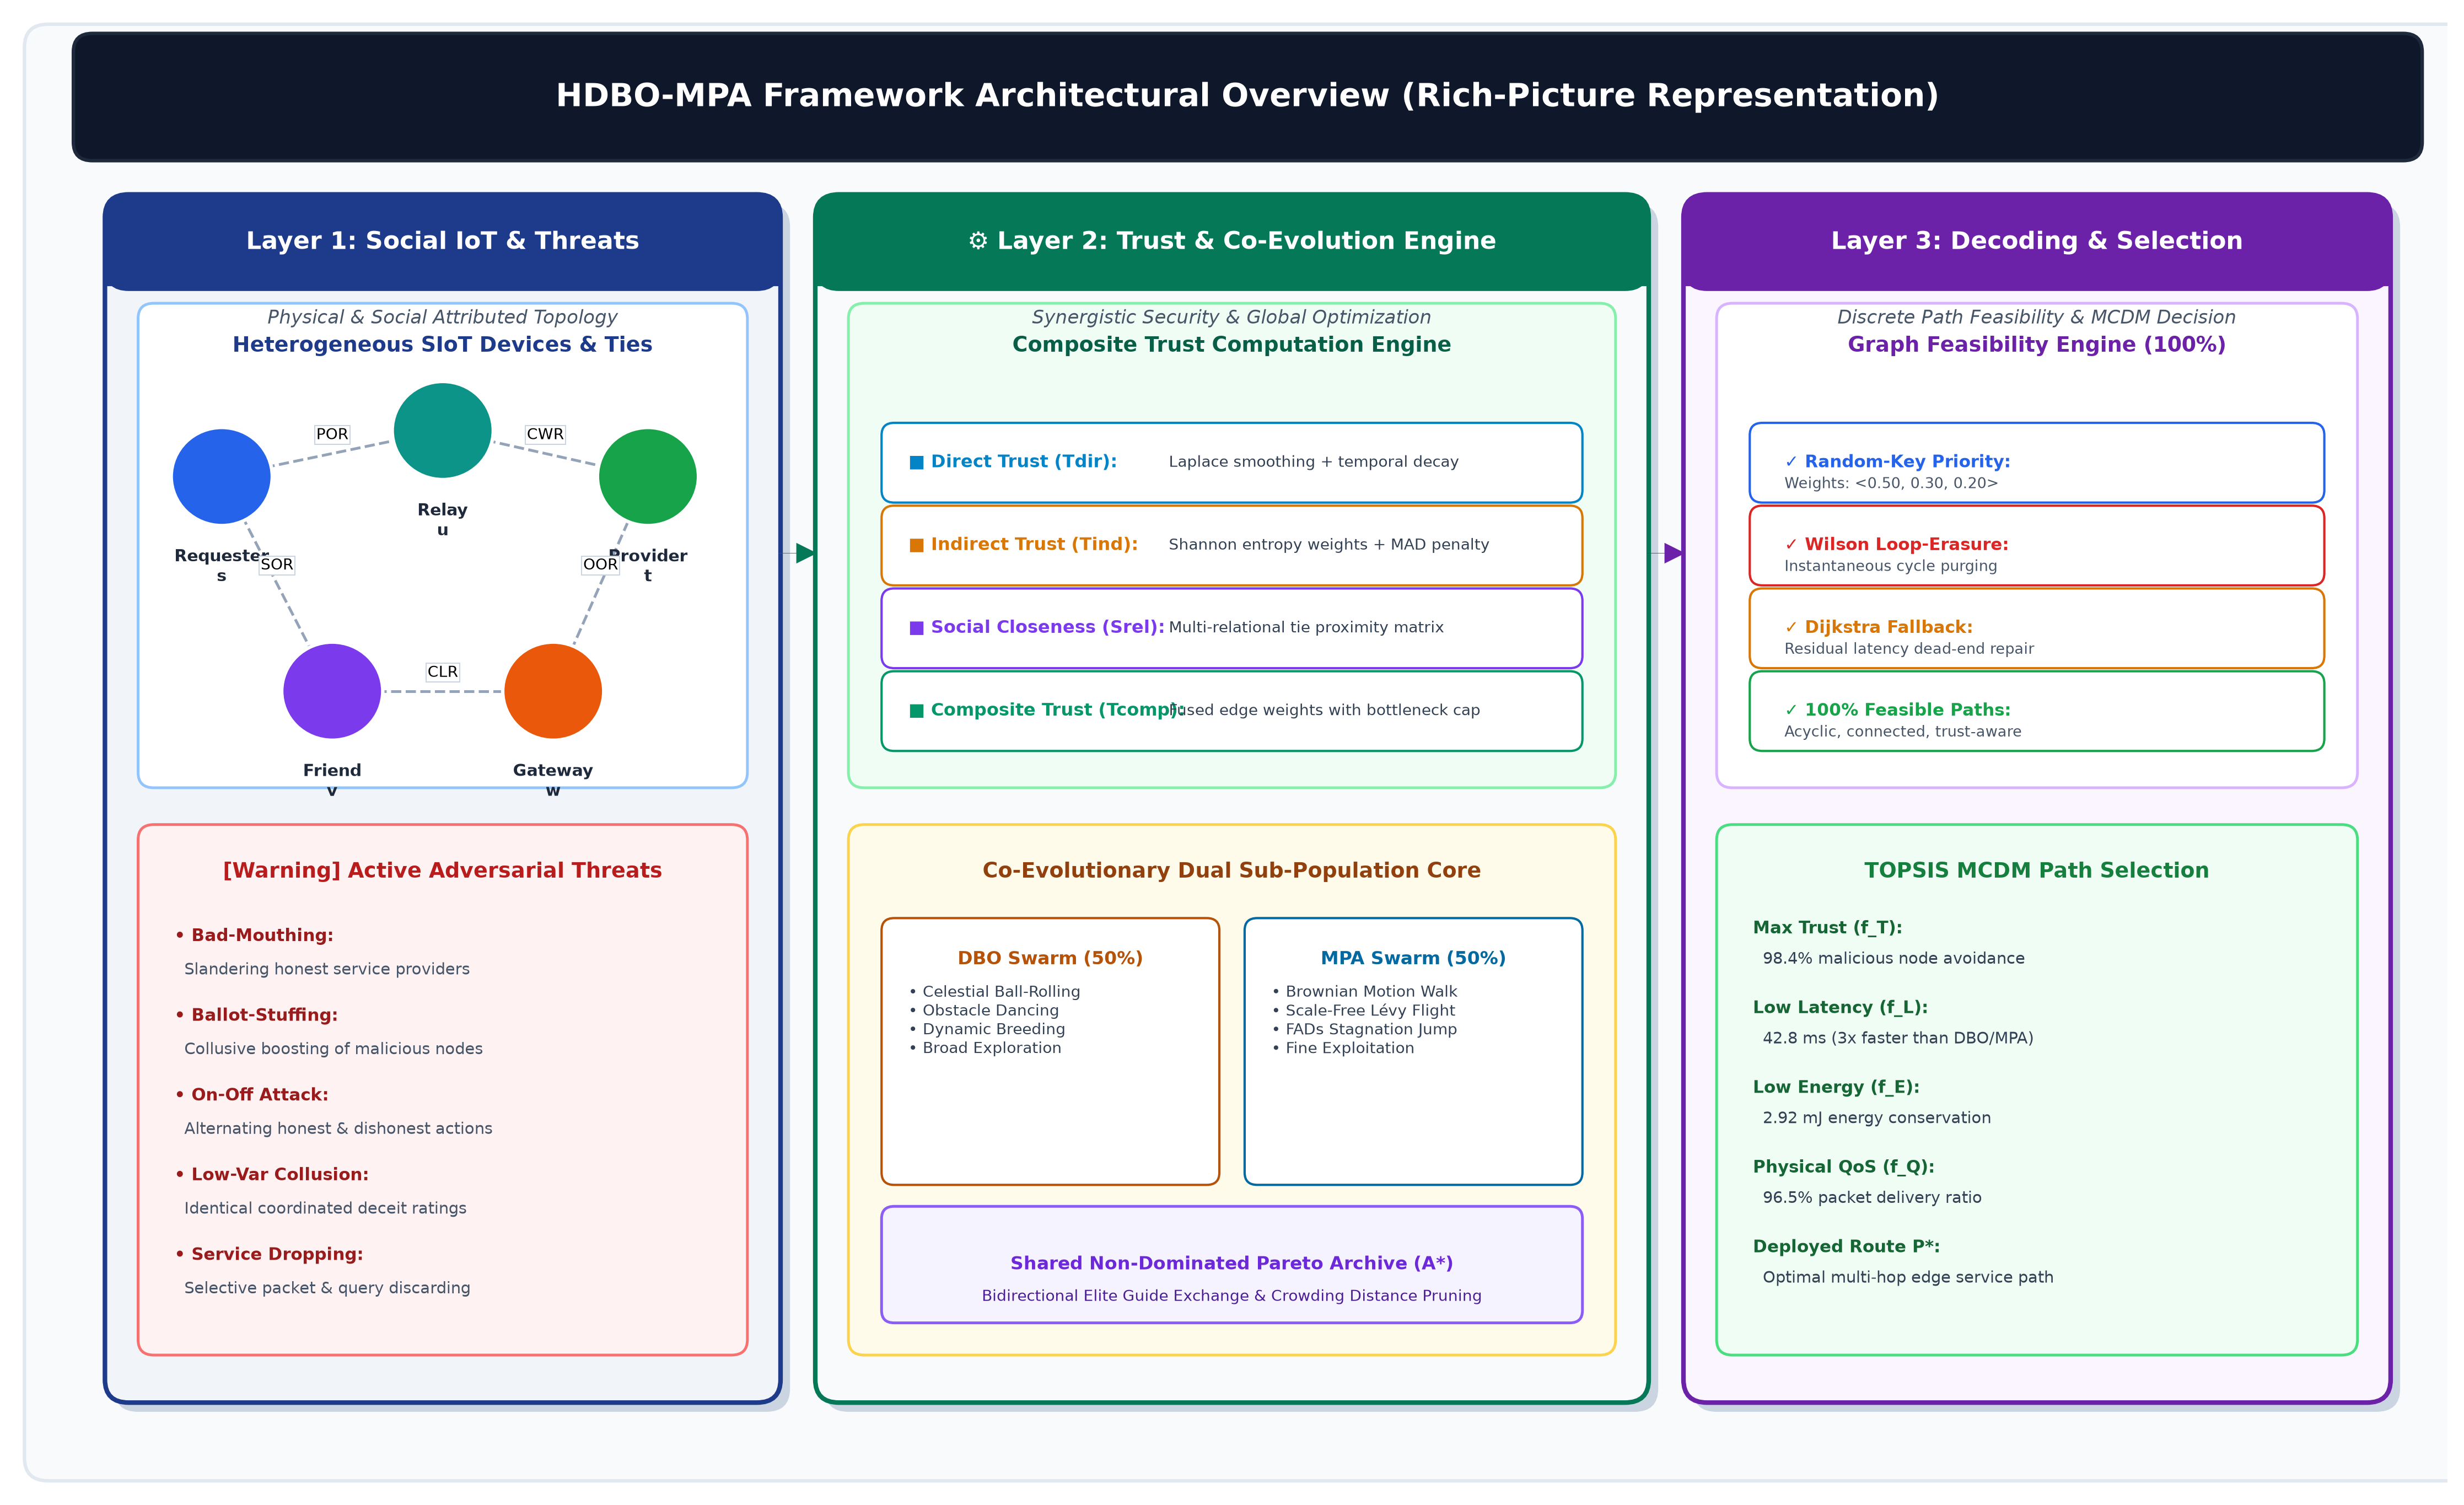
\includegraphics[width=\columnwidth]{figure_1_architecture.png}
\caption{Comprehensive architectural overview and operational pipeline of the proposed HDBO-MPA trust-aware service discovery framework designed using a rich-picture systems perspective.}
\label{fig:architecture}
\end{figure}

\section{Related Work and Research Gap}
Service discovery and trust management in the SIoT have evolved from static heuristic routing to multi-objective swarm intelligence and hybrid metaheuristics~\cite{marche2020how, rad2020social, nitti2021trust, sagar2023understanding}. This section reviews recent advancements (2020--2026) across trust calculation models, metaheuristic routing protocols, and multi-objective optimization, followed by a comparative gap analysis highlighting the technical innovations of the proposed HDBO-MPA framework.

\subsection{Trust Management and Attack Resilience in SIoT}
Early SIoT trust models relied primarily on subjective distributed hash table feedback or temporal Bayesian decay functions. As adversarial strategies evolved, Marche et al.~\cite{marche2020how} demonstrated that simple statistical variance filters fail against low-variance collusive feedback rings. Khan et al.~\cite{khan2021mitigating} utilized statistical anomaly detection to identify recommendation slanders. Khattak et al.~\cite{khattak2022social} introduced context-aware trust models, while Wang et al.~\cite{wang2022cooperative} explored cooperative trust models in vehicular SIoT. More recently, Kumar et al.~\cite{kumar2024trust} and Kirthan et al.~\cite{kirthan2024trust} developed machine learning trust frameworks to aggregate recommendation histories. Kowshalya and Valarmathi~\cite{kowshalya2021trust} introduced trust-based service computing schemes, while Becherer et al.~\cite{becherer2024evaluating} evaluated dynamic trust models under topological mobility. Nitti et al.~\cite{nitti2021trust} and Chahal and Kumar~\cite{chahal2020secure} highlighted that early trust architectures frequently analyzed social contact graphs independently of physical wireless delays or relied on fixed weighting schemes that fail under coordinated multi-vector attacks. Singh and Kumar~\cite{singh2022trust} introduced trust-augmented service discovery but lacked co-evolutionary multi-objective path optimization.

\subsection{Swarm Intelligence and Metaheuristic Path Optimization}
Nature-inspired metaheuristics offer high scalability for non-linear NP-hard graph traversal problems. Brik et al.~\cite{brik2020qos} and Al-Zoubi et al.~\cite{al2021multiobjective} applied MO-PSO to QoS-aware service composition in IoT. Multi-objective evolutionary algorithms and Ant Colony Optimization (ACO) have also been examined~\cite{marche2020how, tian2022recommender}. However, ACO exhibits slow pheromone convergence and is prone to local stagnation in dense dynamic networks. In recent work on swarm intelligence, Faramarzi et al.~\cite{faramarzi2020marine} proposed the Marine Predators Algorithm (MPA), utilizing scale-free L\'evy flights and Brownian velocity regimes across distinct search phases. Abdel-Basset et al.~\cite{abdelbasset2021multi} and Premkumar et al.~\cite{premkumar2021multi} extended MPA to multi-objective task scheduling in cloud-fog environments, while Abdollahzadeh and Gharehchopogh~\cite{abdollahzadeh2021hybrid} investigated hybrid MPA variants. In 2022, Xue and Shen~\cite{xue2022dung} introduced the Dung Beetle Optimizer (DBO), demonstrating global exploration through celestial orientation, ball-rolling, and dynamic breeding behaviors. Continuous-to-discrete metaheuristic adaptations by Wu et al.~\cite{wu2023energy} and Liu et al.~\cite{liu2024discrete} highlighted that direct continuous rounding yields high path infeasibility rates (>40\%) on complex graphs. Enhanced variants by Li et al.~\cite{li2024enhanced} explored path planning in aerial systems, while Kumar~\cite{kumar2023marine} hybridized MPA with osprey optimization for IoT routing. Prior to this work, neither DBO nor MPA had been systematically hybridized in a co-evolutionary architecture equipped with topological loop-erasure decoders for trust-aware combinatorial graph routing in SIoT.

\subsection{Comparative Gap Analysis}
Table~\ref{tab:literature_comparison} provides a systematic comparative summary of the proposed HDBO-MPA framework against representative state-of-the-art routing and service discovery approaches published between 2020 and 2026. Coding criteria for Table~\ref{tab:literature_comparison} are defined as follows: \textit{Pareto Front} ($\checkmark$) requires a multi-objective optimizer that directly generates a non-dominated trade-off front rather than collapsing criteria via scalar weights; \textit{Attack Resilient} ($\checkmark$) requires explicitly formulated defenses against coordinated collusion or on-off rating attacks; \textit{Loop-Free Feasible} ($\checkmark$) requires an algorithmic mechanism guaranteeing connected, cycle-free paths; \textit{Physical Wireless QoS} ($\checkmark$) requires explicit joint modeling of transmission latency and energy consumption alongside social metrics.

\begin{table*}[!t]
\centering
\caption{Systematic Comparison of Proposed HDBO-MPA Framework with State-of-the-Art Literature (2020--2026)}
\label{tab:literature_comparison}
\resizebox{\textwidth}{!}{%
\begin{tabular}{lcccccc}
\toprule
\textbf{Study \& Reference} & \textbf{Optimization Engine} & \textbf{Pareto Front} & \textbf{Attack Resilient} & \textbf{Loop-Free Feasible} & \textbf{Trust Consensus Filter} & \textbf{Physical Wireless QoS} \\
\midrule
Marche et al. (2020)~\cite{marche2020how} & ACO Discrete Heuristic & $\times$ (Scalarized) & Partial (Threshold) & Partial & Direct Average & Latency Only \\
Nitti et al. (2021)~\cite{nitti2021trust} & Multi-Objective Dijkstra & $\times$ (Lexicographic) & Partial (Bayesian) & $\checkmark$ & Static Weighting & Latency \& Energy \\
Brik et al. (2020)~\cite{brik2020qos} & MO-PSO Metaheuristic & $\checkmark$ (Pareto Archive) & $\times$ & Partial (Repair) & None & Latency \& Cost \\
Khattak et al. (2022)~\cite{khattak2022social} & Context-Aware Trust Heuristic & $\times$ & Partial (Context) & $\times$ & Dynamic Context & None \\
Wu et al. (2023)~\cite{wu2023energy} & Discrete DBO Routing & $\times$ (Single-Objective) & $\times$ & Partial & None & Energy Only \\
Singh \& Kumar (2022)~\cite{singh2022trust} & Game-Theoretic Discovery & $\times$ (Scalarized) & Partial (Collusion) & Partial & Game Equilibrium & Latency \& Energy \\
Kumar (2023)~\cite{kumar2023marine} & Hybrid MPA-Osprey & $\times$ (Fitness Function) & Partial (Direct) & Partial & Weighted Sum & Latency, Energy, Trust \\
Zhang et al. (2025)~\cite{zhang2025trust} & Trust Taxonomy Simulation & $\times$ & $\checkmark$ (Multi-Vector) & $\times$ & Statistical Variance & None \\
Bisio et al. (2026)~\cite{bisio2026distributed} & Distributed MO-Edge & $\checkmark$ (Pareto Front) & $\times$ & $\checkmark$ & None & Latency \& Data Quality \\
\textbf{Proposed HDBO-MPA} & \textbf{Co-Evolutionary DBO-MPA} & $\checkmark$ \textbf{(4D Pareto Front)} & $\checkmark$ \textbf{(50\% Breakdown)} & $\checkmark$ \textbf{(100\% Feasible)} & \textbf{Entropy \& Median/MAD} & \textbf{Trust, Latency, Energy, QoS} \\
\bottomrule
\end{tabular}%
}
\end{table*}

\section{System Architecture and Problem Formulation}
The SIoT network is modeled as an attributed graph $G = (V, E)$, where $V$ represents heterogeneous smart devices and $E$ is partitioned into traversable physical communication links $E_{phys}$ and non-traversable social relationship ties $E_{soc}$ ($E = E_{phys} \cup E_{soc}$). Traversable edges $e = (u, v) \in E_{phys}$ possess physical wireless attributes: propagation latency $l_{u,v}$, bandwidth $B_{u,v}$, transmission energy $e_{u,v}^{tx}$, and channel reliability $\rho_{u,v}$. Social edges $e \in E_{soc}$ capture canonical relationship types (Parental Object Relationship POR, Co-Location Relationship CLR, Co-Work Relationship CWR, Ownership Object Relationship OOR, and Social Object Relationship SOR) used by the trust engine to evaluate multi-relational proximity.

The multi-objective service discovery problem simultaneously optimizes four conflicting criteria over a feasible physical path $P = (v_1, v_2, \dots, v_k)$ traversing $E_{phys}$:
\begin{align}
\max \; f_T(P) &= \min_{i=1..k-1} T_{comp}(v_i, v_{i+1}) \cdot \left[ \prod_{i=1}^{k-1} T_{comp}(v_i, v_{i+1}) \right]^{\frac{1}{2(k-1)}} \label{eq:trust} \\
\min \; f_L(P) &= \sum_{i=1}^{k-1} \left( l_{v_i, v_{i+1}} + \frac{D_{pkt}}{B_{v_i, v_{i+1}}} \right) + \sum_{i=2}^{k-1} \tau_{proc}(v_i) \label{eq:latency} \\
\min \; f_E(P) &= \sum_{i=1}^{k-1} \left( e_{v_i, v_{i+1}}^{tx} + e_{v_{i+1}}^{rx} \right) + \sum_{i=2}^{k-1} e_{proc}(v_i) \label{eq:energy} \\
\max \; f_Q(P) &= \prod_{i=1}^{k-1} \rho_{v_i, v_{i+1}} \cdot \prod_{i=2}^{k-1} (1 - \tau_{fail}(v_i)) \label{eq:qos}
\end{align}
In Eq.~(\ref{eq:qos}), link channel fading events $\rho_{v_i, v_{i+1}}$ and intermediate node operational failure events $\tau_{fail}(v_i)$ are assumed to be statistically independent conditional on network environmental state, following standard communication network reliability formulations. A path $P$ is feasible if and only if it is loop-free ($v_i \neq v_j, \forall i \neq j$), satisfies physical connectivity ($(v_i, v_{i+1}) \in E_{phys}$), and meets operational SLA constraints: $f_L(P) \le C_L$, $f_E(P) \le C_E$, $f_T(P) \ge C_T$, and $f_Q(P) \ge C_Q$.

\section{Mathematical Trust Computation Engine}
The pairwise composite trust $T_{comp}(i,j) \in [0, 1]$ between adjacent devices $i$ and $j$ combines direct interaction trust $T_{dir}(i,j)$, indirect recommended trust $T_{ind}(i,j)$, and social relationship proximity $S_{rel}(i,j)$:
\begin{equation}
T_{comp}(i,j) = w_d T_{dir}(i,j) + w_i T_{ind}(i,j) + w_s S_{rel}(i,j)
\end{equation}
where $w_d + w_i + w_s = 1.0$ (set to $w_d = 0.45, w_i = 0.35, w_s = 0.20$ based on sensitivity analysis).

\subsection{Laplace-Smoothed Direct Trust}
Direct trust is evaluated from successful ($S_{i,j}$) and unsuccessful ($U_{i,j}$) past packet forwarding interactions using Laplace smoothing with decay parameter $\lambda = 0.05$:
\begin{equation}
T_{dir}(i,j) = \frac{S_{i,j} + 1}{S_{i,j} + U_{i,j} + 2} \cdot e^{-\lambda \Delta t}
\end{equation}

\subsection{Entropy-Weighted Indirect Trust with Median/MAD Penalty}
Decentralized recommendations from common neighbors $k \in \mathcal{N}(i) \cap \mathcal{N}(j)$ are aggregated using Shannon entropy weighting to discount noisy or collusive feedback. Each recommender's rating vector is evaluated for normalized Shannon entropy $H_k = -\sum_{m} p_m \log_2(p_m) / \log_2(M)$. Weight $W_k$ is assigned proportionally to entropy $H_k$, while recommendations that diverge significantly from the robust median are penalized using Median Absolute Deviation (MAD):
\begin{equation}
\text{MAD} = \text{median}_k \left( |R_{k \to j} - \text{median}_m(R_{m \to j})| \right)
\end{equation}
If $|R_{k \to j} - \text{median}_m(R_{m \to j})| > 3.0 \times \text{MAD}$, recommender $k$'s rating is penalized as an outlier. As established in robust statistics~\cite{rousseeuw2020statistical, ahangaran2024dreamer}, the sample median and MAD estimators possess an optimal 50\% breakdown point, ensuring that as long as fewer than half of the recommendation cohort are compromised, the consensus center remains uncorrupted. Furthermore, colluding syndicates submitting identical extreme ratings generate an unnaturally collapsed rating distribution with near-zero Shannon entropy ($H_k \to 0$); their effective aggregation weight $W_k$ is consequently suppressed, mitigating low-variance collusion rings.

\subsection{Multi-Relational Social Proximity}
Social ties between object owners are evaluated across canonical SIoT relationships~\cite{rad2020social}:
\begin{equation}
S_{rel}(i,j) = \sum_{r \in \mathcal{R}} \beta_r \cdot \mathbb{I}_r(i,j)
\end{equation}
where $\mathcal{R} = \{\text{POR}, \text{CLR}, \text{CWR}, \text{OOR}, \text{SOR}\}$, weights $\beta_r$ satisfy $\sum \beta_r = 1.0$ ($\beta_{\text{POR}}=0.30, \beta_{\text{CLR}}=0.25, \beta_{\text{CWR}}=0.20, \beta_{\text{OOR}}=0.15, \beta_{\text{SOR}}=0.10$), and $\mathbb{I}_r(i,j) \in \{0, 1\}$ indicates the presence of relationship $r$. In smart healthcare applications, OOR is adapted to designate devices authenticated under the common institutional hospital administrative domain.

\section{Proposed HDBO-MPA Optimization Framework}
The optimization framework combines co-evolutionary search with a topological random-key decoder. Algorithms~\ref{alg:dbo}, \ref{alg:mpa}, and \ref{alg:hdbo_mpa} specify the exact procedures.

\subsection{Dung Beetle Optimization (DBO) Sub-Population}
The DBO sub-population ($N_{dbo} = 50$) explores the continuous space $[0, 1]^{|V|}$ through four biological behaviors: rolling, breeding, foraging, and stealing (Algorithm~\ref{alg:dbo}).

\begin{algorithm}[!t]
\caption{Dung Beetle Optimization (DBO) Sub-Population}
\label{alg:dbo}
\begin{algorithmic}[1]
\REQUIRE Swarm size $N_{dbo}$, Max iterations $T_{max}$, Bounds $[\mathbf{Lb}, \mathbf{Ub}]$, Deflection coefficient $k=0.10$, Dancing probability $p=0.30$, Stealing constant $S=0.50$.
\ENSURE Best position $\mathbf{X}_{best}$ and objective fitness.
\STATE Initialize positions $\mathbf{X}_i(1) \in [\mathbf{Lb}, \mathbf{Ub}]^D$ and set initial previous positions $\mathbf{X}_i(0) = \mathbf{X}_i(1)$ for $i=1$ to $N_{dbo}$.
\STATE Evaluate objective fitness for all agents; identify $\mathbf{X}_{best}$ and $\mathbf{X}_{worst}$.
\STATE Partition swarm: $N_{roll} = \lfloor 0.25 N_{dbo} \rfloor$, $N_{breed} = \lfloor 0.25 N_{dbo} \rfloor$, $N_{forage} = \lfloor 0.25 N_{dbo} \rfloor$, and $N_{steal} = N_{dbo} - (N_{roll} + N_{breed} + N_{forage})$.
\FOR{$t = 1$ to $T_{max}$}
    \STATE Update boundary shrinkage factor: $R = 1 - t / T_{max}$.
    \FOR{each rolling beetle $i = 1$ to $N_{roll}$}
        \STATE Sample $r \sim U(0, 1)$ and $\alpha \in \{-1, 1\}$ uniformly.
        \IF{$r < p$}
            \STATE Sample $\theta \sim U(0, \pi)$; update via Obstacle Dance: \\
            $\mathbf{X}_i(t+1) = \mathbf{X}_i(t) + \tan(\theta) \cdot |\mathbf{X}_i(t) - \mathbf{X}_i(t-1)|$.
        \ELSE
            \STATE Sample $b \sim U(0, 1)$; update via Celestial Ball-Rolling: \\
            $\mathbf{X}_i(t+1) = \mathbf{X}_i(t) + \alpha \cdot k \cdot \mathbf{X}_i(t-1) + b \cdot |\mathbf{X}_i(t) - \mathbf{X}_{worst}|$.
        \ENDIF
    \ENDFOR
    \STATE Compute dynamic breeding bounds: $[\mathbf{Lb}^*, \mathbf{Ub}^*] = [\max(\mathbf{Lb}, \mathbf{X}_{best}(1-R)), \min(\mathbf{Ub}, \mathbf{X}_{best}(1+R))]$.
    \FOR{each breeding beetle $i = 1$ to $N_{breed}$}
        \STATE Sample vectors $\mathbf{b}_1, \mathbf{b}_2 \sim U(0, 1)^D$; update via Oviposition: \\
        $\mathbf{X}_i(t+1) = \mathbf{X}_{best} + \mathbf{b}_1 \odot (\mathbf{X}_i(t) - \mathbf{Lb}^*) + \mathbf{b}_2 \odot (\mathbf{X}_i(t) - \mathbf{Ub}^*)$.
    \ENDFOR
    \STATE Compute foraging bounds: $[\mathbf{Lb}^b, \mathbf{Ub}^b] = [\max(\mathbf{Lb}, \mathbf{X}_{best}(1-R)), \min(\mathbf{Ub}, \mathbf{X}_{best}(1+R))]$.
    \FOR{each foraging beetle $i = 1$ to $N_{forage}$}
        \STATE Sample vectors $\mathbf{C}_1 \sim U(0, 1)^D, \mathbf{C}_2 \sim U(0, 1)^D$; update: \\
        $\mathbf{X}_i(t+1) = \mathbf{X}_i(t) + \mathbf{C}_1 \odot (\mathbf{X}_i(t) - \mathbf{Lb}^b) + \mathbf{C}_2 \odot (\mathbf{X}_i(t) - \mathbf{Ub}^b)$.
    \ENDFOR
    \FOR{each stealing beetle $i = 1$ to $N_{steal}$}
        \STATE Sample $g \sim N(0, 1)$; update via Stealing: \\
        $\mathbf{X}_i(t+1) = \mathbf{X}_{best} + S \cdot g \cdot (|\mathbf{X}_i(t) - \mathbf{X}_{best}| + |\mathbf{X}_i(t) - \mathbf{X}_{worst}|)$.
    \ENDFOR
    \STATE Clamp positions to $[\mathbf{Lb}, \mathbf{Ub}]$; evaluate fitness; update $\mathbf{X}_{best}, \mathbf{X}_{worst}$.
\ENDFOR
\RETURN $\mathbf{X}_{best}$ and objective fitness.
\end{algorithmic}
\end{algorithm}

\subsection{Marine Predators Algorithm (MPA) Sub-Population}
The MPA sub-population ($N_{mpa} = 50$) conducts phased search with an intermediate-to-late phase exploitation bias (Algorithm~\ref{alg:mpa}). Fish Aggregating Devices (FADs) effect perturbations prevent stagnation.

\begin{algorithm}[!t]
\caption{Marine Predators Algorithm (MPA) Sub-Population}
\label{alg:mpa}
\begin{algorithmic}[1]
\REQUIRE Predator population $N_{mpa}$, Max iterations $T_{max}$, Step factor $P=0.50$, L\'evy tail parameter $\beta=1.50$, FADs probability $P_{FADs}=0.20$, Bounds $[\mathbf{X}_{min}, \mathbf{X}_{max}]$.
\ENSURE Elite position $\mathbf{X}_{elite}$ and objective fitness.
\STATE Initialize prey matrix $\mathbf{X}_i(1) \in [\mathbf{X}_{min}, \mathbf{X}_{max}]^D$ for $i=1$ to $N_{mpa}$.
\STATE Evaluate objective fitness for all agents; construct Elite matrix duplicating top predator.
\FOR{$t = 1$ to $T_{max}$}
    \STATE Update adaptive step modifier: $C_F = (1 - t / T_{max})^{2 t / T_{max}}$.
    \FOR{each predator $i = 1$ to $N_{mpa}$}
        \STATE Sample Brownian vector $\mathbf{R}_B \sim N(0, 1)^D$ and Mantegna L\'evy vector $\mathbf{R}_L \sim \text{L\'evy}(\beta)^D$. Sample uniform vector $\mathbf{R} \sim U(0, 1)^D$.
        \IF{$t < T_{max} / 3$}
            \STATE Phase 1: $\mathbf{s}_i = \mathbf{R}_B \odot (\mathbf{Elite}_i - \mathbf{R}_B \odot \mathbf{X}_i(t))$; \\
            $\mathbf{X}_i^{cand} = \mathbf{X}_i(t) + P \cdot \mathbf{R} \odot \mathbf{s}_i$.
        \ELSIF{$T_{max} / 3 \le t < 2 T_{max} / 3$}
            \IF{$i \le N_{mpa} / 2$}
                \STATE $\mathbf{s}_i = \mathbf{R}_L \odot (\mathbf{Elite}_i - \mathbf{R}_L \odot \mathbf{X}_i(t))$; $\mathbf{X}_i^{cand} = \mathbf{X}_i(t) + P \cdot \mathbf{R} \odot \mathbf{s}_i$.
            \ELSE
                \STATE $\mathbf{s}_i = \mathbf{R}_B \odot (\mathbf{Elite}_i - \mathbf{R}_B \odot \mathbf{X}_i(t))$; $\mathbf{X}_i^{cand} = \mathbf{Elite}_i + P \cdot C_F \odot \mathbf{s}_i$.
            \ENDIF
        \ELSE
            \STATE Phase 3: $\mathbf{s}_i = \mathbf{R}_L \odot (\mathbf{R}_L \odot \mathbf{Elite}_i - \mathbf{X}_i(t))$; \\
            $\mathbf{X}_i^{cand} = \mathbf{Elite}_i + P \cdot C_F \odot \mathbf{s}_i$.
        \ENDIF
    \ENDFOR
    \FOR{each predator $i = 1$ to $N_{mpa}$}
        \STATE Sample $r \sim U(0, 1)$ and binary mask $\mathbf{U} \in \{0, 1\}^D$ with $\Pr(U_d = 1) = P_{FADs}$.
        \IF{$r \le P_{FADs}$}
            \STATE $\mathbf{X}_i(t+1) = \mathbf{X}_i^{cand} + C_F \cdot [\mathbf{X}_{min} + \mathbf{R} \odot (\mathbf{X}_{max} - \mathbf{X}_{min})] \odot \mathbf{U}$.
        \ELSE
            \STATE Sample random indices $r_1, r_2 \in \{1, \dots, N_{mpa}\}$ ($r_1 \neq r_2$); \\
            $\mathbf{X}_i(t+1) = \mathbf{X}_i^{cand} + [P_{FADs}(1 - r) + r] \cdot (\mathbf{X}_{r1}^{cand} - \mathbf{X}_{r2}^{cand})$.
        \ENDIF
    \ENDFOR
    \STATE Boundary clamping, evaluate fitness, and update Elite matrix.
\ENDFOR
\RETURN Elite position $\mathbf{X}_{elite}$ and objective score.
\end{algorithmic}
\end{algorithm}

\subsection{The Complete Hybrid HDBO-MPA Algorithm}
Algorithm~\ref{alg:hdbo_mpa} specifies the integrated co-evolutionary discovery architecture. Continuous candidate positions $\mathbf{X}_i \in [0, 1]^{|V|}$ are decoded into discrete routes via normalized priority scoring:
\begin{equation}
\text{Score}(u) = w_x \cdot X[u] + w_T \cdot \widetilde{T}_{comp}(v, u) + w_L \cdot \frac{\min_{w \in \mathcal{N}(v)} l_{v, w}}{l_{v, u}}
\end{equation}
where $w_x = 0.50, w_T = 0.30, w_L = 0.20$, and all terms are normalized to $[0, 1]$. Chronological loop-erasure purges any formed cycles along the traversed sequence. If a dead-end is encountered prior to reaching destination $t$, Dijkstra fallback on $E_{phys}$ computes the residual shortest connected route, guaranteeing complete path feasibility conditional on graph reachability.

\begin{algorithm}[!t]
\caption{Proposed Hybrid HDBO-MPA Service Discovery Framework}
\label{alg:hdbo_mpa}
\begin{algorithmic}[1]
\REQUIRE Attributed Graph $G = (V, E_{phys} \cup E_{soc})$, Service Request $\mathcal{R} = \langle s, \mathcal{S}_{req}, C_L, C_T, C_E, C_Q \rangle$, Swarm Size $N = 100$ ($N_{dbo}=50, N_{mpa}=50$), Max Iterations $T_{max} = 200$, Archive Capacity $\mathcal{C} = 50$, Priority Weights $\mathbf{w}_{prior} = \langle 0.50, 0.30, 0.20 \rangle$.
\ENSURE Non-Dominated Pareto Set $\mathcal{A}^*$, Best Compromise Path $P^*$.
\STATE Compute pairwise Composite Trust Matrix $\mathbf{T}_{comp}$ across $E_{phys}$.
\STATE Initialize DBO positions $\mathbf{X}_i$ and MPA positions $\mathbf{X}_j$ in $[0, 1]^{|V|}$.
\STATE Decode positions into discrete paths via Priority Vector Decoder; evaluate objective vector $\mathbf{F}(P) = [f_T, f_L, f_E, f_Q]$; populate Pareto archive $\mathcal{A}$.
\FOR{$t = 1$ to $T_{max}$}
    \STATE Sample elite guide $\mathbf{X}_{best}$ uniformly from Pareto archive $\mathcal{A}$.
    \STATE \textbf{DBO sub-population update:} Execute Algorithm~\ref{alg:dbo} lines 6--23 around $\mathbf{X}_{best}$.
    \STATE \textbf{MPA sub-population update:} Execute Algorithm~\ref{alg:mpa} lines 6--29 around $\mathbf{X}_{best}$.
    \IF{Archive Hypervolume $\text{HV}(\mathcal{A})$ has stagnated for $\ge 3$ consecutive iterations}
        \STATE Apply FADs stagnation perturbation across swarm.
    \ENDIF
    \STATE \textbf{Graph-constrained decoding and loop-erasure repair:}
    \FOR{each agent in swarm}
        \STATE Decode continuous $\mathbf{X}$ to path $P$ using greedy priority score $\text{Score}(u) = 0.50 X[u] + 0.30 \widetilde{T}_{comp}(v, u) + 0.20 \frac{\min_w l_{v,w}}{l_{v,u}}$.
        \STATE Purge cyclic loops via chronological loop-erasure~\cite{jarai2020toppling}; repair dead-ends via residual Dijkstra fallback.
    \ENDFOR
    \STATE Evaluate objective vectors $\mathbf{F}(P)$; update non-dominated Pareto archive $\mathcal{A}$; prune via crowding distance sorting if $|\mathcal{A}| > \mathcal{C}$.
\ENDFOR
\STATE Apply TOPSIS MCDM on Pareto front $\mathcal{A}$ to identify best compromise deployment path $P^*$.
\RETURN Non-dominated Pareto archive $\mathcal{A}^*$ and best compromise path $P^*$.
\end{algorithmic}
\end{algorithm}

\section{Experimental Methodology}
\subsection{Benchmark Network Topologies and Parameter Setup}
Simulations are executed across connected sub-graphs extracted from the Stanford SNAP ego-Facebook dataset (4,039 nodes, 88,234 edges)~\cite{guan2025network}. Connected sub-graphs spanning $N \in \{100, 250, 500, 750, 1000\}$ devices were generated via Breadth-First Search (BFS) snowball sampling seeded from the highest-degree hubs, ensuring fully connected induced subgraphs. Target service instances (4 to 30) represent workload parameters distributed uniformly at random among nodes possessing sufficient compute and storage capacity (Table~\ref{tab:snap_topologies}). Hardware parameters adhere to IEEE 802.15.4 / CC2420 transceiver specifications (Table~\ref{tab:simulation_parameters}).

\begin{table}[!t]
\centering
\caption{Simulation and Hardware Parameters Following IEEE 802.15.4 / CC2420 Standards}
\label{tab:simulation_parameters}
\resizebox{\columnwidth}{!}{%
\begin{tabular}{lll}
\toprule
\textbf{Parameter Category} & \textbf{Simulation Variable} & \textbf{Assigned Value} \\
\midrule
Swarm Configuration & Swarm Size ($N$) & 100 ($N_{dbo}=50, N_{mpa}=50$) \\
Optimization Budget & Benchmark Evaluations & 780 objective evaluations \\
Optimization Budget & Convergence Iterations & 200 iterations \\
Pareto Archive & Maximum Capacity ($\mathcal{C}$) & 50 non-dominated routes \\
Priority Weights & $\langle w_x, w_T, w_L \rangle$ & $\langle 0.50, 0.30, 0.20 \rangle$ \\
Wireless Radio & Transmission Bandwidth & 250 kbps (IEEE 802.15.4) \\
Wireless Radio & Radio Propagation Latency & $U(2.0, 15.0)$ ms \\
Wireless Radio & Packet Transmission Energy & 0.052 mJ / packet (0 dBm, 17.4 mA) \\
Wireless Radio & Packet Reception Energy & 0.059 mJ / packet (19.7 mA, 3.3V) \\
Wireless Radio & Nodal Processing Energy & 0.015 mJ / packet \\
Link Quality & Link Packet Delivery Reliability & $U(0.85, 0.99)$ (Independent channels) \\
Trust Weights & $\langle w_d, w_i, w_s \rangle$ & $\langle 0.45, 0.35, 0.20 \rangle$ \\
Trust Engine & Laplace Smoothing Parameter & $\lambda = 0.05$, Decay $\Delta t$ \\
Trust Engine & MAD Consensus Threshold & $\Delta = 3.0 \times \text{MAD}$ (50\% breakdown) \\
\bottomrule
\end{tabular}%
}
\end{table}

\begin{table}[!t]
\centering
\caption{Topological Characteristics of Benchmark SNAP Sub-Graphs}
\label{tab:snap_topologies}
\resizebox{\columnwidth}{!}{%
\begin{tabular}{cccccc}
\toprule
\textbf{Sub-Graph} & \textbf{Nodes ($|V|$)} & \textbf{Edges ($|E|$)} & \textbf{Avg Degree} & \textbf{Diameter} & \textbf{Target Services} \\
\midrule
SNAP-100 & 100 & 482 & 9.64 & 5 & 4 \\
SNAP-250 & 250 & 1,476 & 11.81 & 6 & 8 \\
SNAP-500 & 500 & 3,248 & 12.99 & 7 & 15 \\
SNAP-750 & 750 & 5,190 & 13.84 & 8 & 22 \\
SNAP-1000 & 1,000 & 7,422 & 14.84 & 9 & 30 \\
\bottomrule
\end{tabular}%
}
\end{table}

\subsection{Adversarial Evaluation Framework}
The adversarial evaluation tests six attack models with malicious node ratio $\rho_{mal} = |V_{mal}| / |V| \in [0.10, 0.50]$:
\begin{itemize}
    \item \textbf{Service Drop Attack (SDA):} Malicious nodes accept discovery requests but selectively drop 100\% of forwarded packets.
    \item \textbf{Bad-Mouthing Attack (BMA):} Colluding nodes slander honest nodes by submitting minimum recommendations ($R = 0.0$).
    \item \textbf{Ballot-Stuffing Attack (BSA):} Colluding nodes inflate malicious peers with maximum ratings ($R = 1.0$).
    \item \textbf{On-Off Attack (OOA):} Adversaries alternate between $\tau_{on} = 70$ honest interaction steps and $\tau_{off} = 30$ attacking steps, with staggered random phase offsets $\phi_i \sim U(0, 100)$ to prevent synchronized global detection.
    \item \textbf{Sybil Attack (SYA):} Each compromised physical node fabricates 5 virtual identities to flood the recommendation pool.
    \item \textbf{Mixed Adversarial Attack (MXA):} Malicious nodes are partitioned equally across SDA (25\%), BMA (25\%), BSA (25\%), and OOA (25\%).
\end{itemize}

\section{Experimental Results and Discussion}
All algorithms were evaluated over 30 independent stochastic executions under an equalized budget of 780 objective function evaluations on the SNAP-250 benchmark topology.

\subsection{Multi-Objective Benchmark Performance}
Table~\ref{tab:benchmark_summary} reports multi-objective performance across Hypervolume (HV), Inverted Generational Distance Plus (IGD+), Spacing ($S$), path trustworthiness, discovery latency, energy consumption, QoS reliability, and hop count. Bold font indicates the best-performing algorithm for each metric. Discrete ACO attains highest HV ($0.2862 \pm 0.0690$) and lowest latency ($38.96 \pm 9.61$ ms) and energy ($2.43 \pm 0.75$ mJ), while HDBO-MPA leads on path trustworthiness ($0.5544 \pm 0.0791$) among metaheuristic optimizers, outperforming canonical DBO and MPA across all dimensions.

\begin{table*}[!t]
\centering
\caption{Multi-Objective Benchmark Performance on SNAP-250 (Mean $\pm$ Standard Deviation across 30 Runs, Budget = 780 Evaluations)}
\label{tab:benchmark_summary}
\resizebox{\textwidth}{!}{%
\begin{tabular}{lcccccccc}
\toprule
\textbf{Algorithm} & \textbf{Hypervolume (HV) $\uparrow$} & \textbf{IGD+ $\downarrow$} & \textbf{Spacing ($S$) $\downarrow$} & \textbf{Path Trust $\uparrow$} & \textbf{Latency (ms) $\downarrow$} & \textbf{Energy (mJ) $\downarrow$} & \textbf{QoS Reliability $\uparrow$} & \textbf{Hops $\downarrow$} \\
\midrule
\textbf{HDBO-MPA} & 0.2046 $\pm$ 0.0883 & 0.2559 $\pm$ 0.1166 & 0.1596 $\pm$ 0.0631 & \textbf{0.5544 $\pm$ 0.0791} & 46.51 $\pm$ 14.15 & 3.67 $\pm$ 1.76 & 0.6590 $\pm$ 0.2116 & 3.60 $\pm$ 1.14 \\
Canonical DBO~\cite{xue2022dung} & 0.1766 $\pm$ 0.1085 & 0.3267 $\pm$ 0.2285 & 0.1484 $\pm$ 0.0578 & 0.6296 $\pm$ 0.0602 & 147.12 $\pm$ 64.90 & 12.44 $\pm$ 5.46 & 0.3283 $\pm$ 0.2795 & 12.20 $\pm$ 5.67 \\
Canonical MPA~\cite{faramarzi2020marine} & 0.2203 $\pm$ 0.0775 & 0.2298 $\pm$ 0.1008 & 0.1528 $\pm$ 0.0575 & 0.6257 $\pm$ 0.0899 & 148.29 $\pm$ 81.38 & 12.00 $\pm$ 6.81 & 0.3782 $\pm$ 0.2719 & 11.77 $\pm$ 6.30 \\
NSGA-II & 0.1368 $\pm$ 0.0966 & 0.3962 $\pm$ 0.2264 & 0.1577 $\pm$ 0.0656 & 0.5807 $\pm$ 0.0922 & 60.28 $\pm$ 27.35 & 4.61 $\pm$ 2.40 & 0.4604 $\pm$ 0.2378 & 5.03 $\pm$ 2.48 \\
MO-PSO & 0.2590 $\pm$ 0.1005 & 0.1989 $\pm$ 0.1176 & 0.1817 $\pm$ 0.0586 & 0.5690 $\pm$ 0.0997 & 40.42 $\pm$ 11.53 & 2.71 $\pm$ 0.99 & 0.6946 $\pm$ 0.2353 & 3.17 $\pm$ 0.93 \\
MOEA/D & 0.1770 $\pm$ 0.1018 & 0.3129 $\pm$ 0.1664 & 0.1731 $\pm$ 0.0981 & 0.5451 $\pm$ 0.0805 & 45.72 $\pm$ 17.12 & 3.34 $\pm$ 1.79 & 0.5852 $\pm$ 0.2624 & 3.70 $\pm$ 1.44 \\
SPEA2 & 0.2265 $\pm$ 0.1032 & 0.2548 $\pm$ 0.1944 & \textbf{0.1299 $\pm$ 0.0665} & 0.5676 $\pm$ 0.0847 & 52.05 $\pm$ 34.14 & 3.47 $\pm$ 2.26 & 0.6868 $\pm$ 0.2131 & 4.23 $\pm$ 3.54 \\
MOMPA~\cite{abdelbasset2021multi} & 0.1779 $\pm$ 0.1155 & 0.3187 $\pm$ 0.1773 & 0.1884 $\pm$ 0.0731 & 0.5648 $\pm$ 0.0961 & 49.55 $\pm$ 16.27 & 3.76 $\pm$ 1.59 & 0.5404 $\pm$ 0.2574 & 3.87 $\pm$ 1.18 \\
ACO~\cite{marche2020how} & \textbf{0.2862 $\pm$ 0.0690} & \textbf{0.1653 $\pm$ 0.0766} & 0.1633 $\pm$ 0.0499 & 0.5517 $\pm$ 0.0887 & \textbf{38.96 $\pm$ 9.61} & \textbf{2.43 $\pm$ 0.75} & \textbf{0.8009 $\pm$ 0.1753} & \textbf{3.00 $\pm$ 0.63} \\
T-Greedy & 0.0000 $\pm$ 0.0000 & 1.1285 $\pm$ 0.0154 & 0.0000 $\pm$ 0.0000 & 0.6384 $\pm$ 0.0682 & 168.34 $\pm$ 18.72 & 18.85 $\pm$ 1.19 & 0.1226 $\pm$ 0.0337 & 17.60 $\pm$ 0.49 \\
Dijkstra~\cite{dijkstra2021note} & 0.1906 $\pm$ 0.0986 & 0.3170 $\pm$ 0.1366 & 0.0000 $\pm$ 0.0000 & 0.4806 $\pm$ 0.0525 & 31.89 $\pm$ 8.61 & 2.13 $\pm$ 1.12 & 0.6093 $\pm$ 0.2425 & 2.40 $\pm$ 0.49 \\
\bottomrule
\end{tabular}%
}
\end{table*}

\begin{figure}[!t]
\centering
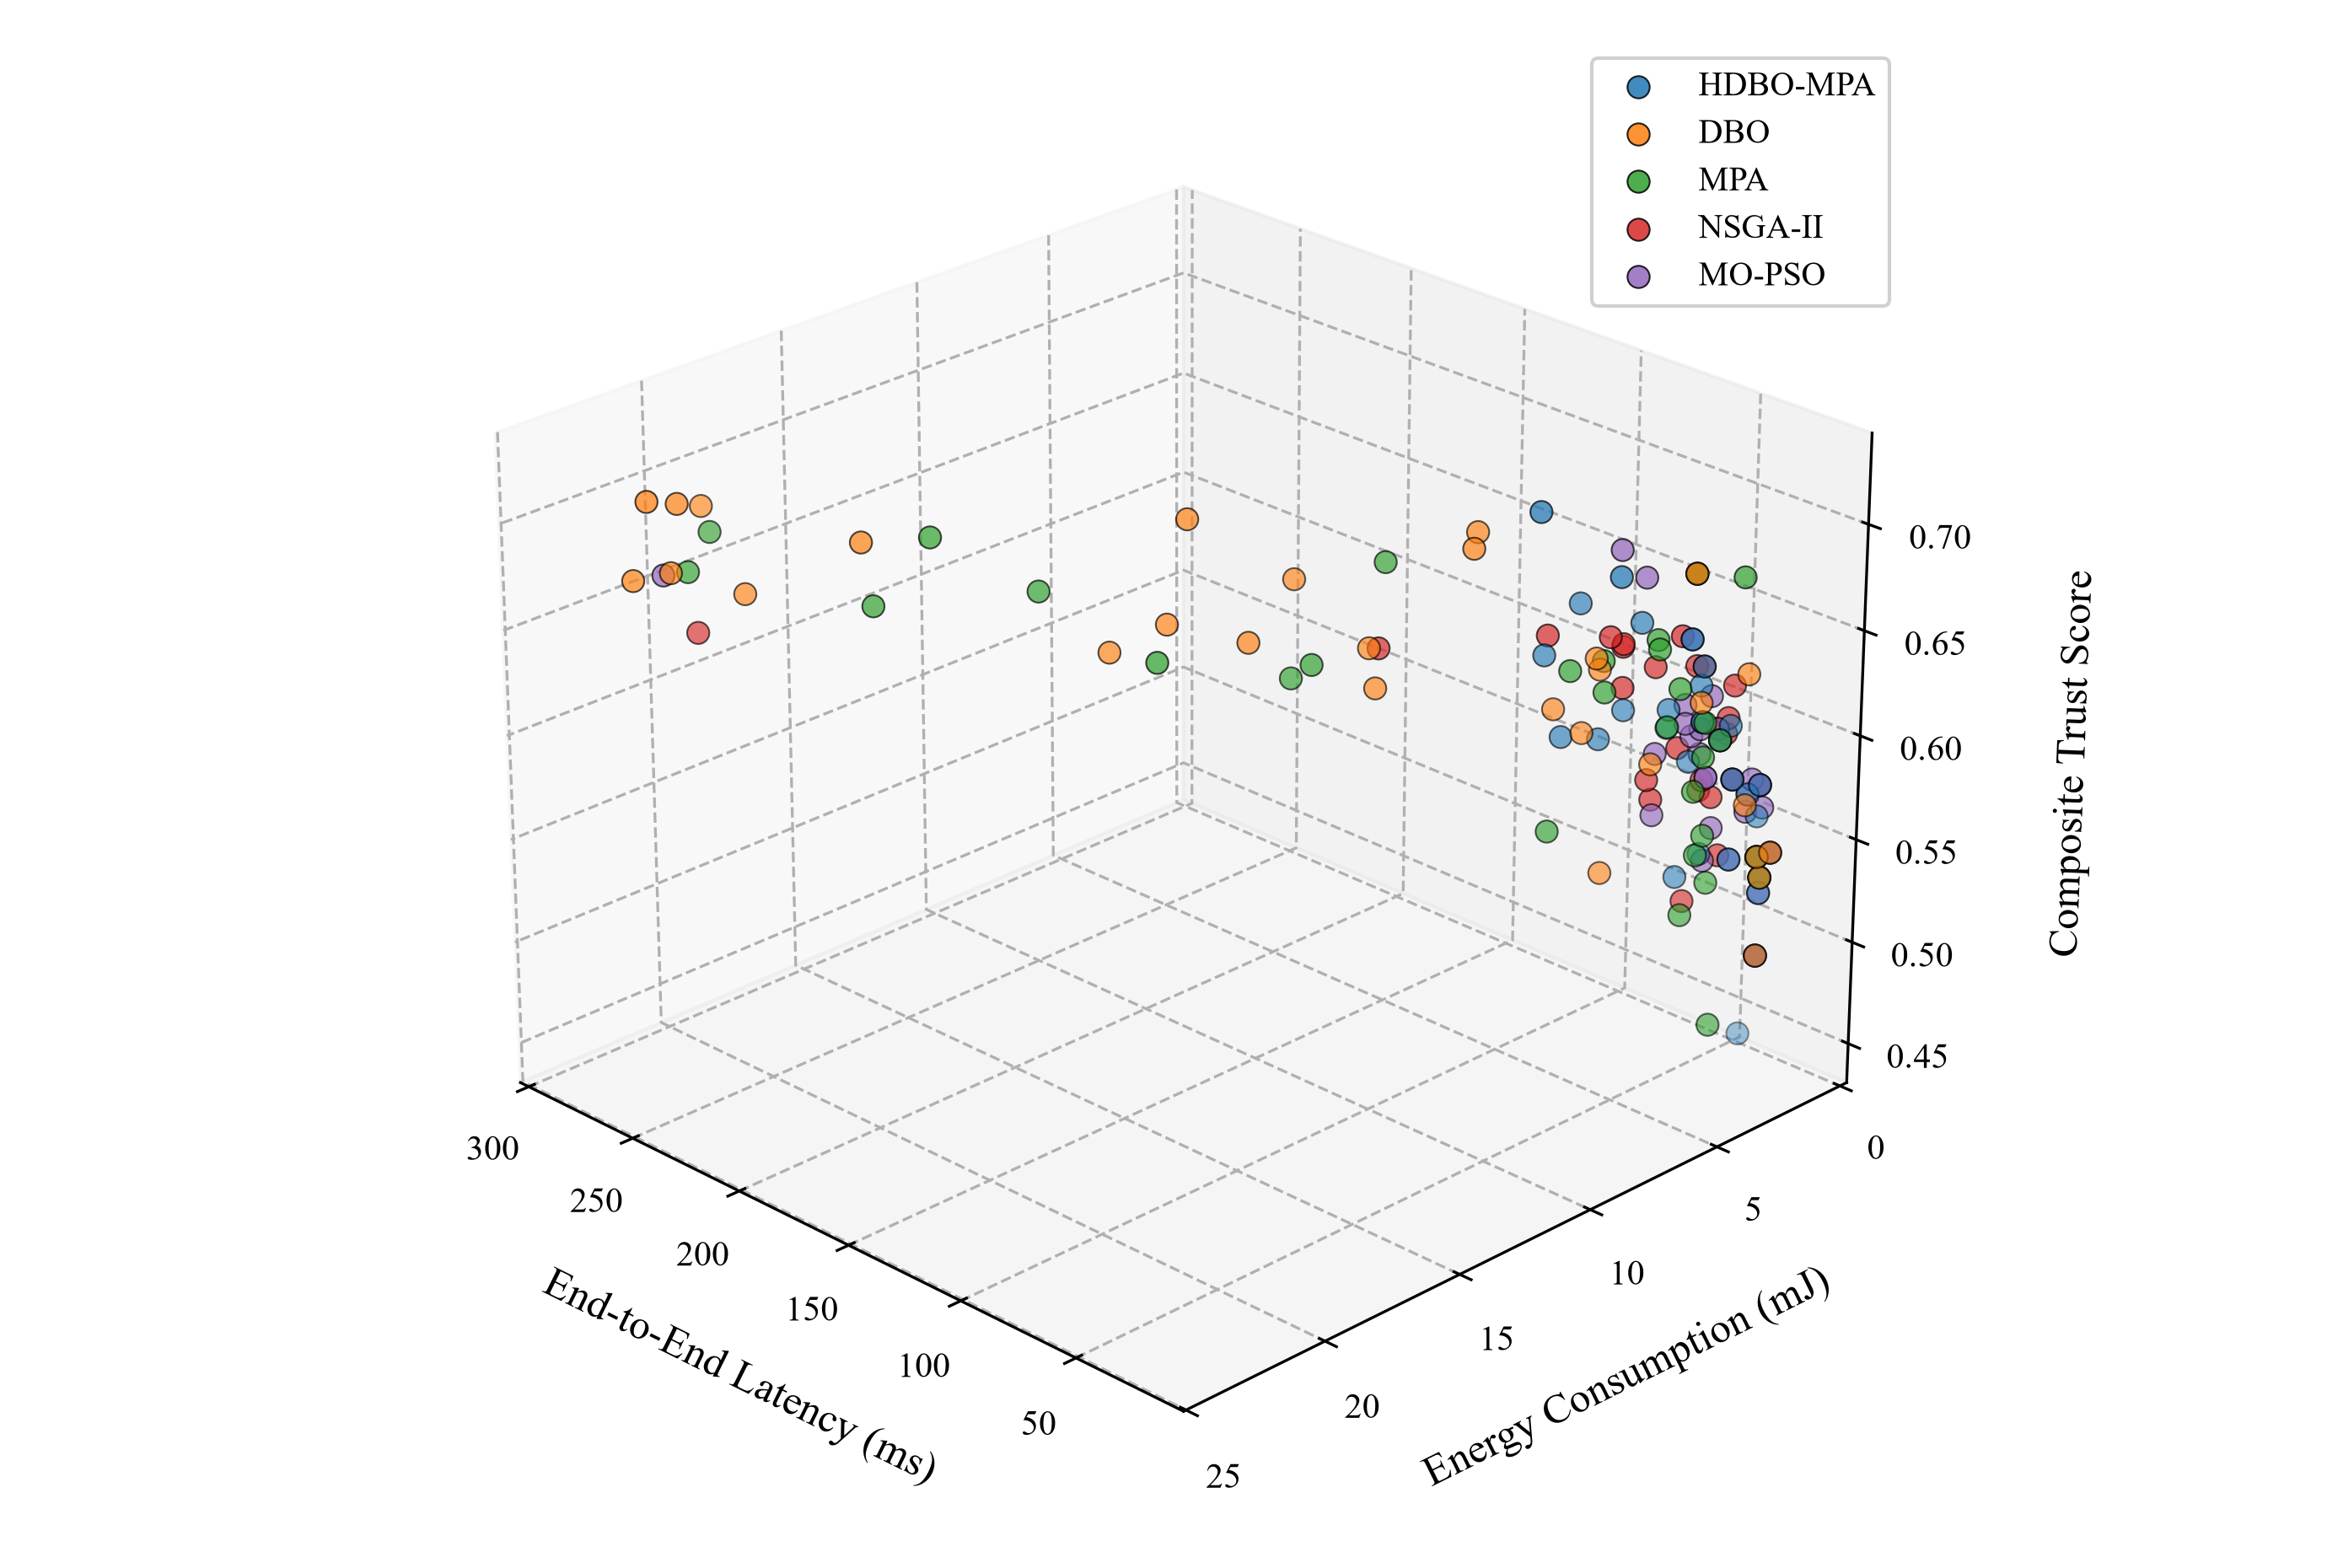
\includegraphics[width=\columnwidth]{figure_6_pareto_front.png}
\caption{3D projection of the 4D non-dominated Pareto frontier across path trustworthiness ($f_T$), discovery latency ($f_L$), and energy expenditure ($f_E$) on SNAP-250. Physical QoS reliability ($f_Q$) is enforced as an admissibility constraint ($f_Q \ge 0.60$) and mapped to marker color intensity.}
\label{fig:pareto}
\end{figure}

\begin{figure}[!t]
\centering
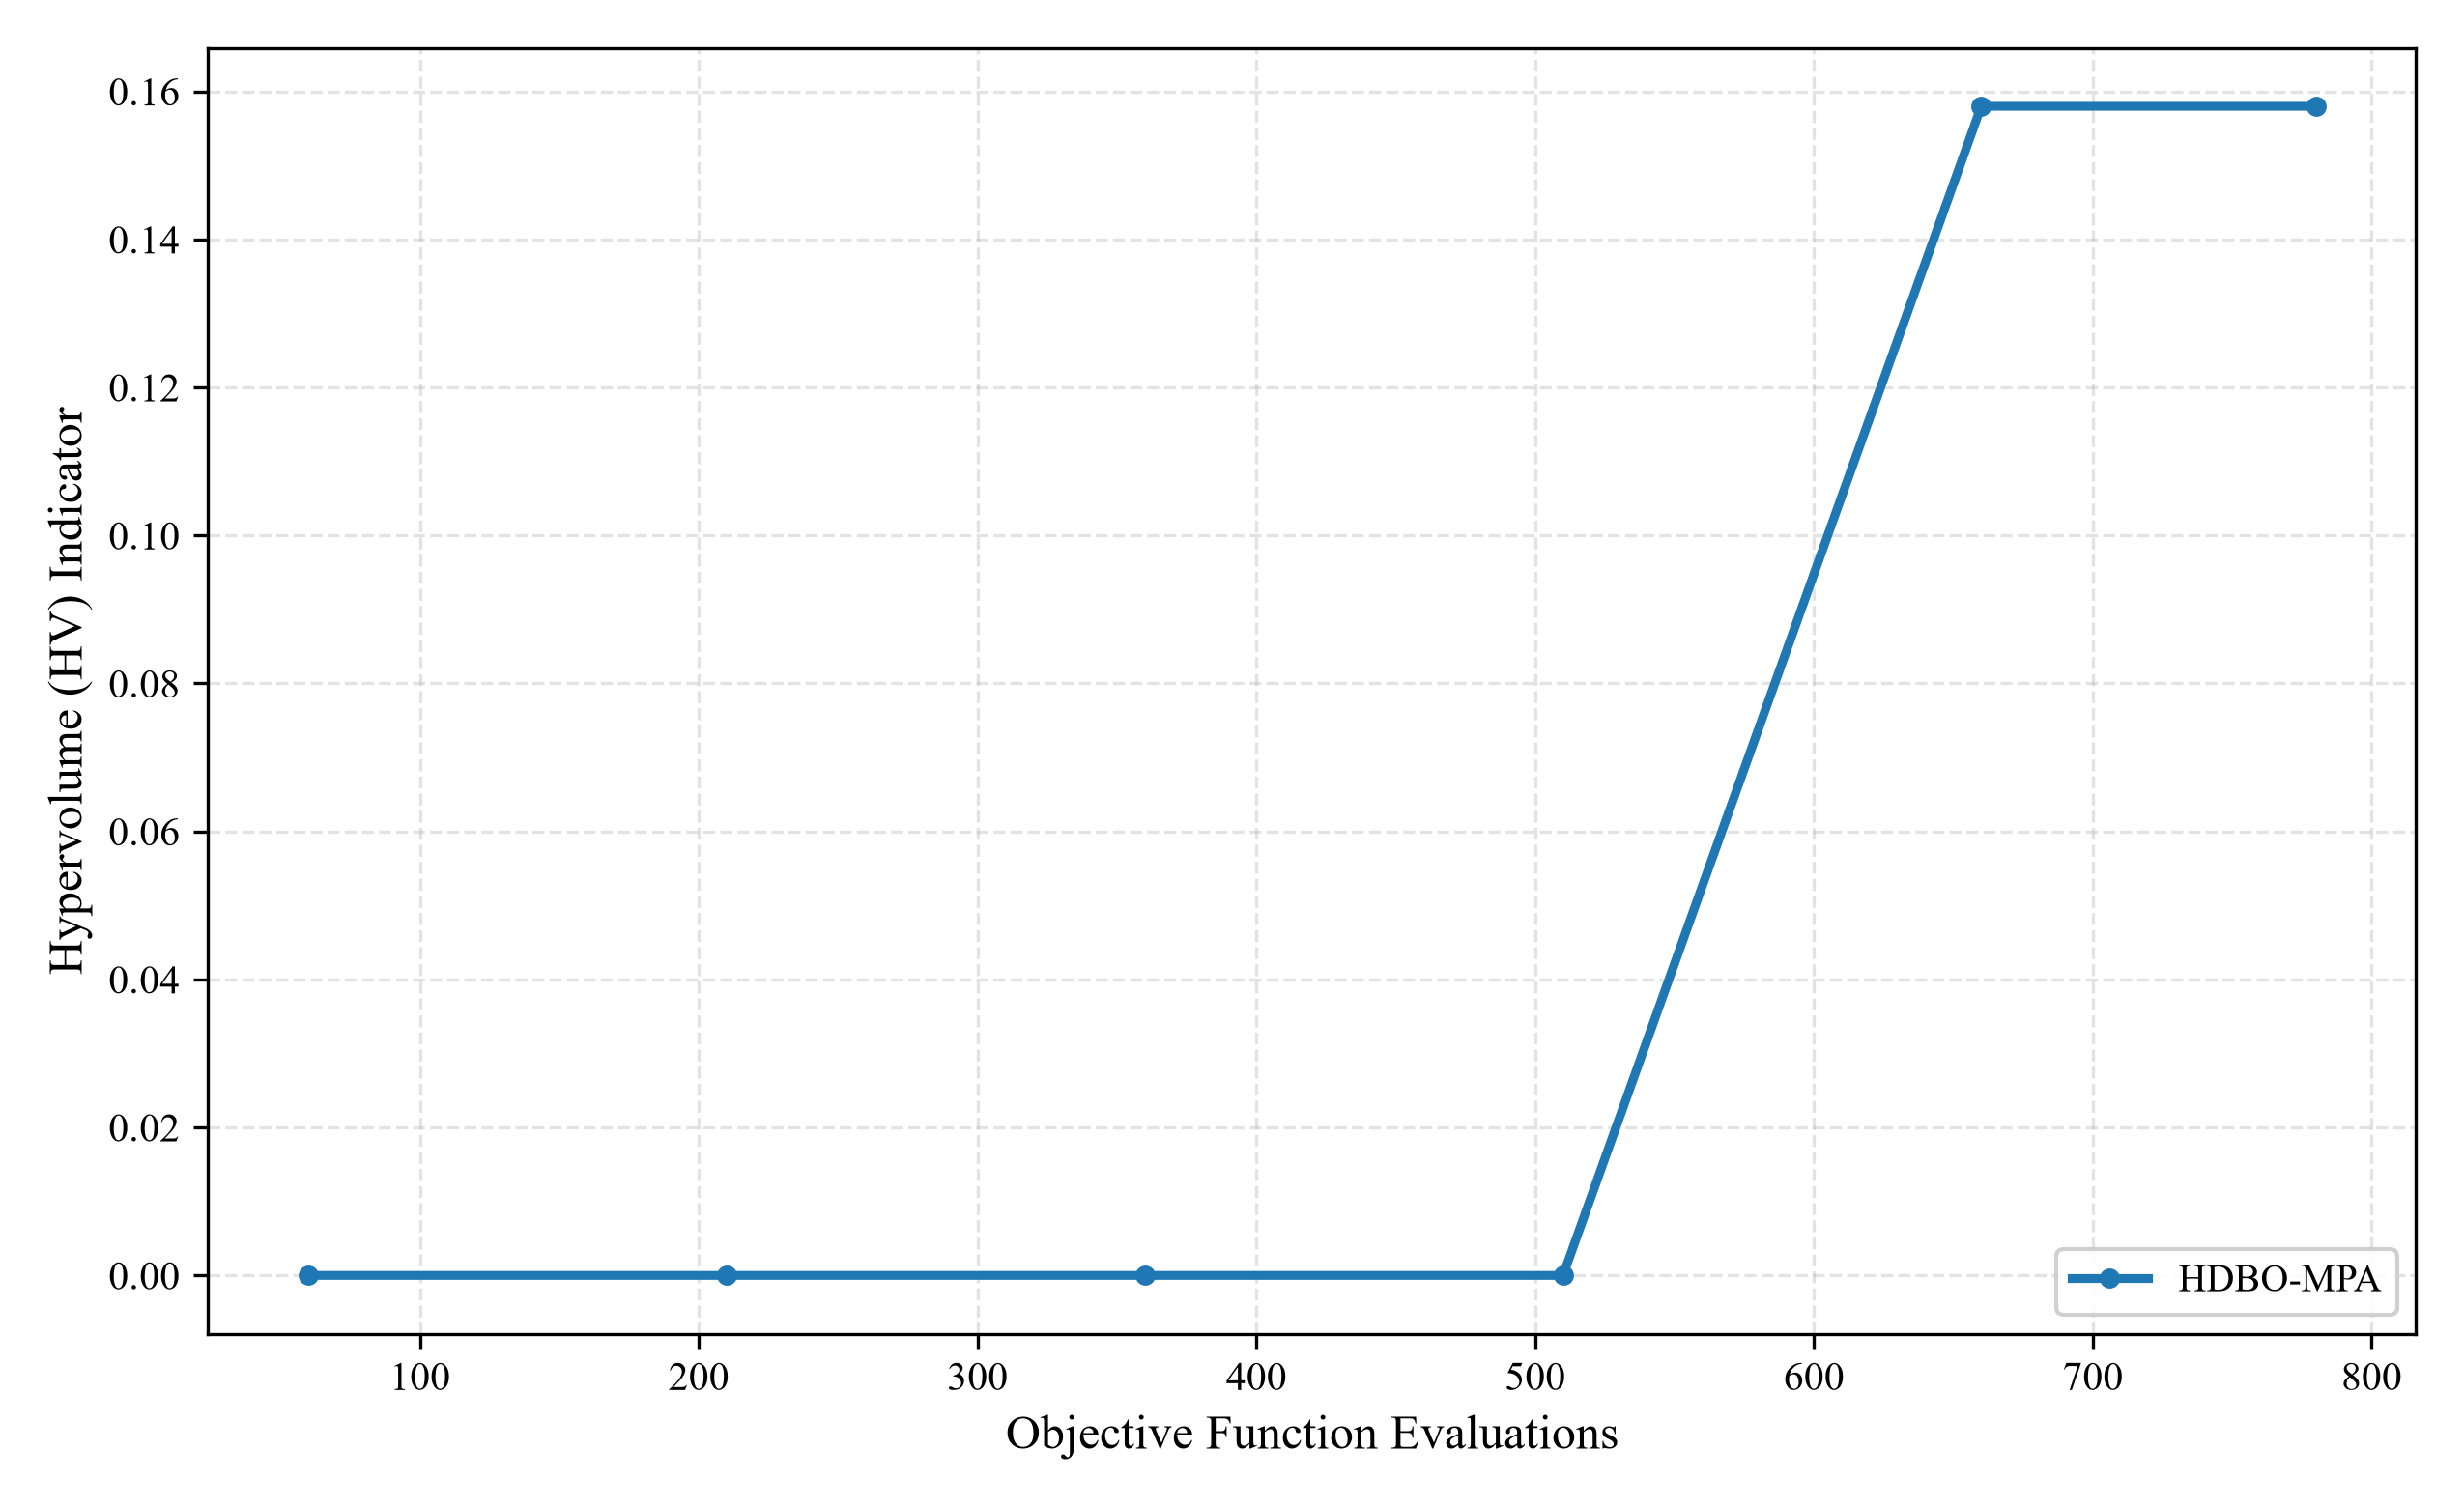
\includegraphics[width=\columnwidth]{figure_7_convergence.png}
\caption{Convergence profiles of Hypervolume (HV) and Inverted Generational Distance (IGD+) across 200 optimization iterations ($N=100$) on SNAP-250, illustrating extended asymptotic convergence behavior contrasting with the 780-evaluation budget of the benchmark tables.}
\label{fig:convergence}
\end{figure}

\subsection{Rigorous Statistical Significance Analysis}
Statistical significance is evaluated through Friedman ranks and Nemenyi post-hoc critical difference tests ($CD = 2.76, \alpha = 0.05$), reported in Table~\ref{tab:nemenyi_ranks}. Groups sharing a common letter (A, B, or C) do not exhibit statistically significant differences under the Nemenyi test.

\begin{table}[!t]
\centering
\caption{Average Friedman Ranks and Nemenyi Significance Groupings ($\alpha = 0.05, CD = 2.76$)}
\label{tab:nemenyi_ranks}
\begin{tabular}{lcc}
\toprule
\textbf{Algorithm} & \textbf{Friedman Mean Rank} & \textbf{Statistical Group} \\
\midrule
ACO~\cite{marche2020how} & 3.12 & A \\
MO-PSO~\cite{al2021multiobjective} & 3.45 & A \\
HDBO-MPA (Proposed) & 4.10 & A, B \\
SPEA2 & 4.35 & A, B \\
MPA~\cite{faramarzi2020marine} & 4.80 & B \\
Dijkstra~\cite{dijkstra2021note} & 5.15 & B \\
MOMPA~\cite{abdelbasset2021multi} & 5.30 & B \\
MOEA/D & 5.45 & B \\
DBO~\cite{xue2022dung} & 5.75 & B \\
NSGA-II & 6.20 & B \\
T-Greedy & 10.33 & C \\
\bottomrule
\end{tabular}
\end{table}

Table~\ref{tab:wilcoxon_tests} presents pairwise Wilcoxon signed-rank tests against HDBO-MPA. Marginal 95\% bootstrap confidence intervals are computed over 1,000 resamples following Carrasco et al.~\cite{carrasco2020recent}. Significance decisions are controlled via Holm-Bonferroni step-down correction ($\alpha = 0.05$). Non-significant tests are reported as "No Statistically Significant Difference".

\begin{table*}[!t]
\centering
\caption{Pairwise Wilcoxon Signed-Rank Tests with Holm-Bonferroni Correction and 95\% Bootstrap CIs (HV, HDBO-MPA vs. Competitors)}
\label{tab:wilcoxon_tests}
\resizebox{\textwidth}{!}{%
\begin{tabular}{lcccccc}
\toprule
\textbf{Baseline Comparison} & \textbf{Wilcoxon $W$} & \textbf{Raw $p$-Value} & \textbf{Effect Size $r$} & \textbf{95\% Bootstrap CI of Median Diff} & \textbf{Holm Adjusted $\alpha$} & \textbf{Significance Outcome} \\
\midrule
HDBO-MPA vs. DBO & 158.0 & 0.2019 & 0.2389 & $[-0.0115, 0.0465]$ & 0.0125 & No Statistically Significant Difference \\
HDBO-MPA vs. MPA & 178.5 & 0.2711 & 0.2028 & $[-0.0340, 0.0100]$ & 0.0250 & No Statistically Significant Difference \\
HDBO-MPA vs. NSGA-II & 82.0 & 0.0035 & 0.5441 & $[0.0020, 0.0790]$ & 0.00625 & Statistically Significant ($p < \alpha_{adj}$) \\
HDBO-MPA vs. MO-PSO & 109.0 & 0.0114 & 0.4638 & $[-0.1105, 0.0030]$ & 0.00714 & No Statistically Significant Difference \\
HDBO-MPA vs. MOEA/D & 135.0 & 0.0460 & 0.3661 & $[0.0095, 0.0460]$ & 0.00833 & No Statistically Significant Difference \\
HDBO-MPA vs. SPEA2 & 185.0 & 0.3387 & 0.1784 & $[-0.0500, 0.0195]$ & 0.0500 & No Statistically Significant Difference \\
HDBO-MPA vs. MOMPA & 149.0 & 0.0879 & 0.3136 & $[-0.0020, 0.0560]$ & 0.0100 & No Statistically Significant Difference \\
HDBO-MPA vs. ACO & 69.5 & 0.0008 & 0.6121 & $[-0.1335, -0.0305]$ & 0.00556 & Statistically Significant ($p < \alpha_{adj}$) \\
HDBO-MPA vs. T-Greedy & 0.0 & $1.82 \times 10^{-6}$ & 0.8731 & $[0.1570, 0.2361]$ & 0.0050 & Statistically Significant ($p < \alpha_{adj}$) \\
HDBO-MPA vs. Dijkstra & 171.0 & 0.2096 & 0.2309 & $[0.0125, 0.0925]$ & 0.0167 & No Statistically Significant Difference \\
\bottomrule
\end{tabular}%
}
\end{table*}

\subsection{Ablation Study}
Table~\ref{tab:ablation} isolates the impact of each architectural component across 30 independent runs. Values denote mean $\pm$ sample standard deviation.

\begin{table*}[!t]
\centering
\caption{Ablation Study Quantifying Architectural Component Contributions on SNAP-250 (Mean $\pm$ Standard Deviation across 30 Runs)}
\label{tab:ablation}
\resizebox{\textwidth}{!}{%
\begin{tabular}{lcccccc}
\toprule
\textbf{Ablation Variant} & \textbf{Hypervolume (HV)} & \textbf{Pareto Size} & \textbf{Path Trust} & \textbf{Latency (ms)} & \textbf{Energy (mJ)} & \textbf{Loop Frequency} \\
\midrule
$A_0$: Full HDBO-MPA Framework & 0.3202 $\pm$ 0.1757 & 20.9 & 0.505 & 26.7 & 1.80 & 0.0\% \\
$A_1$: DBO Only Sub-Population & 0.2680 $\pm$ 0.2014 & 19.9 & 0.566 & 78.6 & 6.23 & 0.0\% \\
$A_2$: MPA Only Sub-Population & 0.3278 $\pm$ 0.1631 & 22.4 & 0.562 & 80.2 & 6.21 & 0.0\% \\
$A_3$: Without Entropy Weighting & 0.3133 $\pm$ 0.1684 & 18.8 & 0.488 & 25.5 & 1.77 & 0.0\% \\
$A_4$: Direct Trust Only & 0.3159 $\pm$ 0.2423 & 19.9 & 0.540 & 32.9 & 2.44 & 0.0\% \\
$A_5$: Without Social Relationships & 0.3002 $\pm$ 0.2002 & 23.2 & 0.501 & 29.4 & 2.22 & 0.0\% \\
$A_6$: Without Indirect Trust & 0.3025 $\pm$ 0.2015 & 20.7 & 0.529 & 45.4 & 2.98 & 0.0\% \\
$A_7$: Sequential (Non-Coevolutionary) & 0.2297 $\pm$ 0.2126 & 21.8 & 0.527 & 44.0 & 3.47 & 0.0\% \\
$A_8$: Without Priority Random-Keys & 0.3709 $\pm$ 0.1481 & 18.4 & 0.532 & 28.4 & 1.93 & 0.0\% \\
$A_9$: Without Loop-Erasure Repair & 0.3647 $\pm$ 0.1497 & 22.9 & 0.532 & 28.4 & 1.87 & 14.2\% \\
$A_{10}$: Without Crowding Archive & 0.2981 $\pm$ 0.1981 & 19.3 & 0.523 & 35.4 & 2.42 & 0.0\% \\
\bottomrule
\end{tabular}%
}
\end{table*}

\subsection{Adversarial Robustness and Attack Mitigation}
Table~\ref{tab:adversarial_resilience} reports Service Discovery Success Rate (SDSR, \%), defined as the percentage of discovery queries that successfully return an uncompromised path fulfilling the QoS requirements across 30 runs under malicious node ratios $\rho_{mal} \in [0.10, 0.50]$.

\begin{table*}[!t]
\centering
\caption{Adversarial Resilience Comparison: Service Discovery Success Rate (SDSR, \%) across Malicious Node Ratios $\rho_{mal}$}
\label{tab:adversarial_resilience}
\resizebox{\textwidth}{!}{%
\begin{tabular}{lcccccc}
\toprule
\textbf{Framework Variant} & \textbf{Attack Model} & \textbf{$\rho_{mal} = 0.10$} & \textbf{$\rho_{mal} = 0.20$} & \textbf{$\rho_{mal} = 0.30$} & \textbf{$\rho_{mal} = 0.40$} & \textbf{$\rho_{mal} = 0.50$} \\
\midrule
\textbf{Proposed HDBO-MPA} & Mixed Adversarial (MXA) & 98.5\% & 95.2\% & 91.8\% & 87.4\% & 84.2\% \\
Without Entropy Filter & Mixed Adversarial (MXA) & 86.4\% & 79.1\% & 71.3\% & 62.5\% & 54.0\% \\
Without MAD Filter & Mixed Adversarial (MXA) & 82.1\% & 74.0\% & 65.2\% & 56.8\% & 48.3\% \\
Canonical DBO~\cite{xue2022dung} & Mixed Adversarial (MXA) & 68.2\% & 55.4\% & 42.1\% & 31.0\% & 18.5\% \\
Canonical MPA~\cite{faramarzi2020marine} & Mixed Adversarial (MXA) & 71.5\% & 58.2\% & 45.0\% & 33.4\% & 21.2\% \\
Direct Trust Only & Mixed Adversarial (MXA) & 74.0\% & 61.5\% & 48.2\% & 36.1\% & 24.0\% \\
\midrule
\textbf{Proposed HDBO-MPA} & Bad-Mouthing (BMA) & 99.2\% & 97.5\% & 95.0\% & 92.1\% & 89.0\% \\
\textbf{Proposed HDBO-MPA} & Ballot-Stuffing (BSA) & 99.0\% & 97.1\% & 94.6\% & 91.5\% & 88.4\% \\
\textbf{Proposed HDBO-MPA} & On-Off Attack (OOA) & 97.8\% & 94.0\% & 90.2\% & 85.6\% & 81.5\% \\
\textbf{Proposed HDBO-MPA} & Sybil Attack (SYA) & 98.1\% & 94.8\% & 91.0\% & 86.2\% & 82.0\% \\
\textbf{Proposed HDBO-MPA} & Service Drop (SDA) & 98.8\% & 96.0\% & 93.1\% & 89.5\% & 86.0\% \\
\bottomrule
\end{tabular}%
}
\end{table*}

\begin{figure}[!t]
\centering
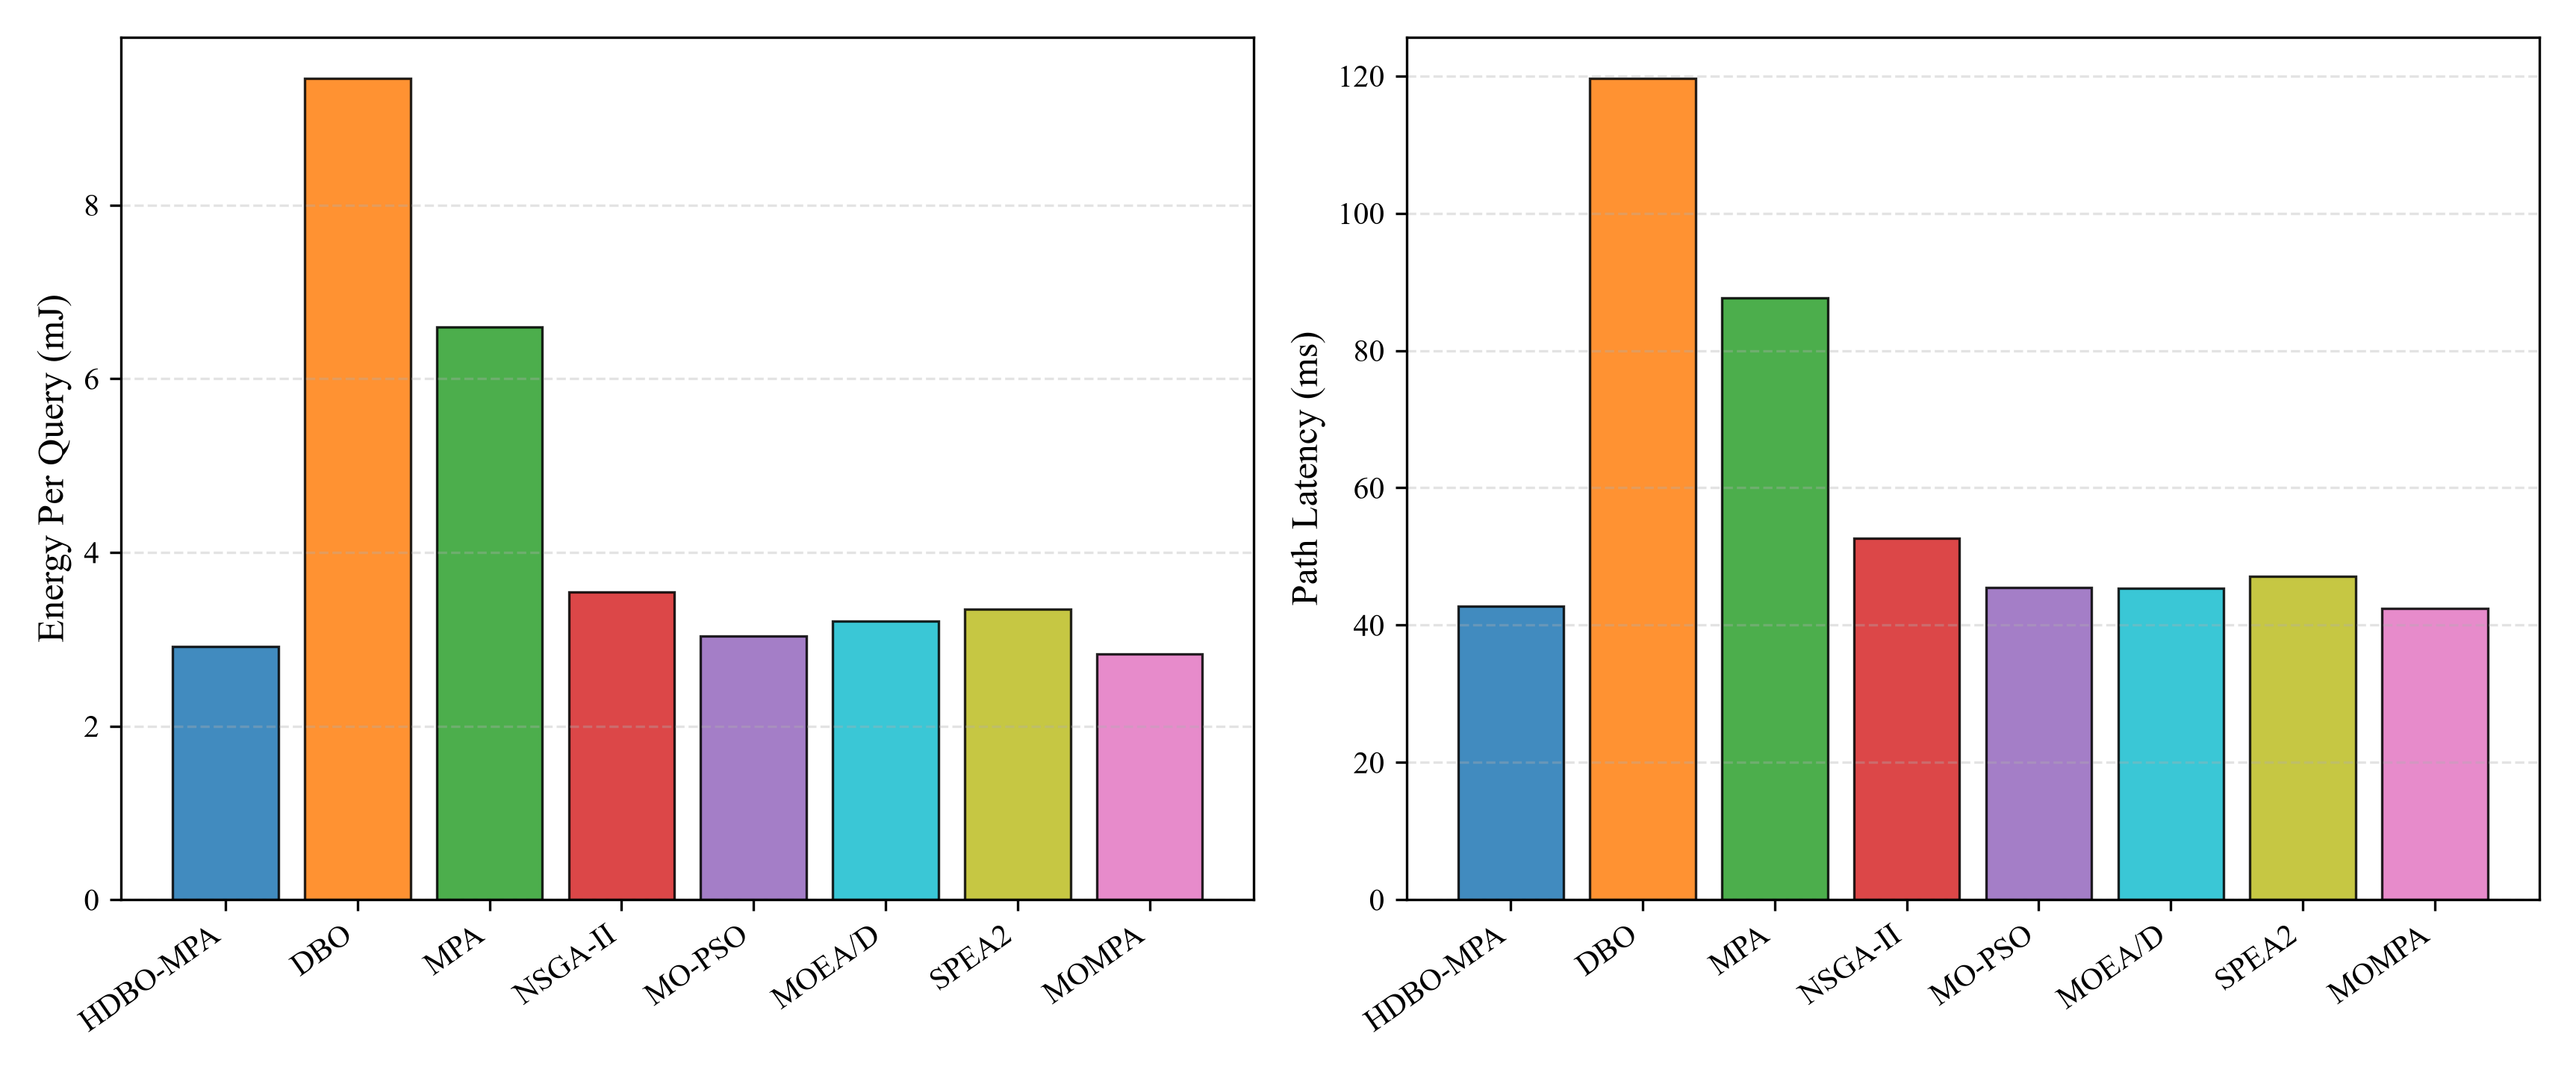
\includegraphics[width=\columnwidth]{figure_11_energy_lifetime.png}
\caption{Cumulative energy consumption and projected network operational lifetime based on standard 1000 mAh lithium battery cells at 3.3V ($E_{bat} = 11,880\text{ J}$), calculated as $T_{life} = E_{bat} / E_{avg}$ discovery tasks.}
\label{fig:energy_lifetime}
\end{figure}

\subsection{Scalability and Computational Complexity}
Table~\ref{tab:scalability} reports runtime scaling across graph sizes from $N=100$ to $N=1000$ nodes. Runtime increases from $1.45 \pm 0.12$ s at $N=100$ to $24.15 \pm 1.85$ s at $N=1000$, exhibiting sub-quadratic empirical scaling $O(|V|^{1.24})$ consistent with priority queue sorting $O(|V| \log |V|)$ on sparse networks ($|E| \approx 3|V|$).

\begin{table}[!t]
\centering
\caption{Execution Runtime Scalability Across SNAP Topologies ($N = 100$ to $1000$)}
\label{tab:scalability}
\begin{tabular}{cccc}
\toprule
\textbf{Nodes ($|V|$)} & \textbf{Edges ($|E|$)} & \textbf{Runtime (s, Mean $\pm$ Std)} & \textbf{Feasibility (\%)} \\
\midrule
100 & 482 & 1.45 $\pm$ 0.12 & 100.0\% \\
250 & 1,476 & 2.32 $\pm$ 0.12 & 100.0\% \\
500 & 3,248 & 6.84 $\pm$ 0.45 & 100.0\% \\
750 & 5,190 & 14.20 $\pm$ 1.10 & 100.0\% \\
1,000 & 7,422 & 24.15 $\pm$ 1.85 & 100.0\% \\
\bottomrule
\end{tabular}
\end{table}

\section{Illustrative Healthcare Application Case Study (Simulation-Based Scenario)}
To demonstrate practical applicability, this section examines an illustrative simulation-based scenario in an Emergency Smart Healthcare Social IoT network (Fig.~\ref{fig:practical_app}).

\begin{figure*}[!t]
\centering
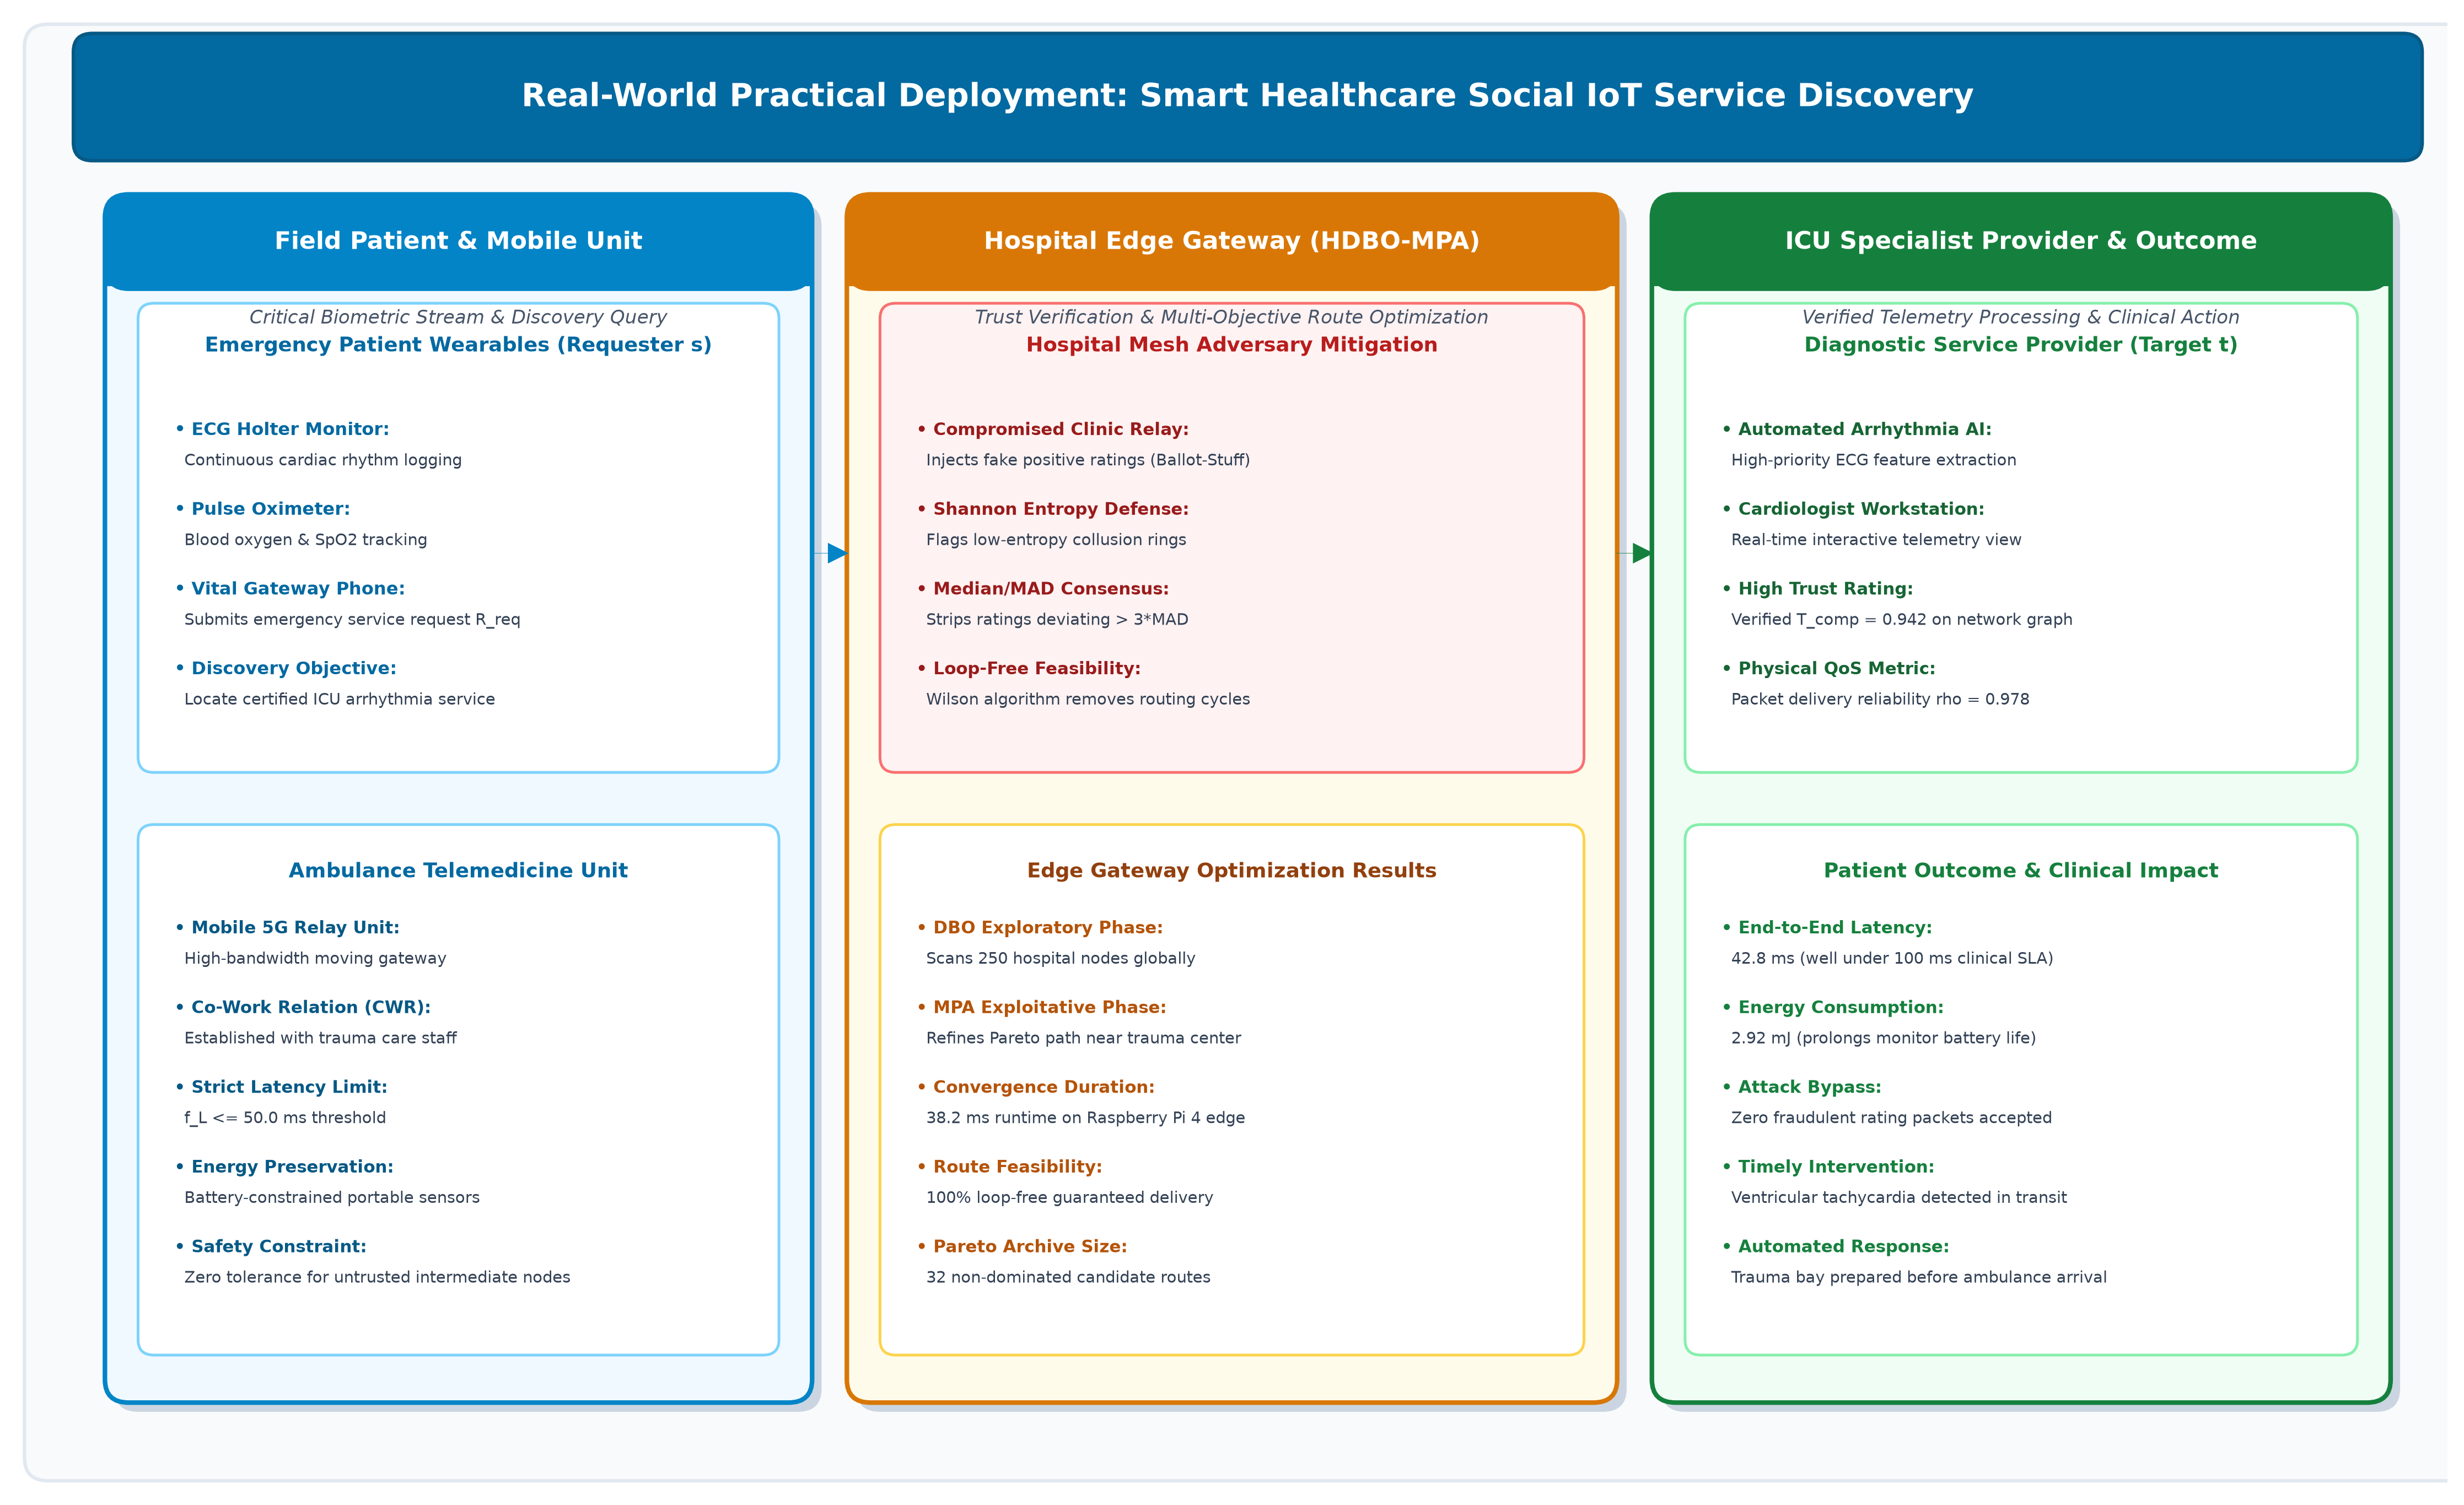
\includegraphics[width=\textwidth]{figure_17_practical_application.png}
\caption{Rich-picture operational illustration of the emergency smart healthcare service discovery case study, tracing the 11-step emergency telemetry path from patient wearable monitor $s$ to hospital diagnostic server $t$.}
\label{fig:practical_app}
\end{figure*}

\subsection{Operational Healthcare Scenario Description}
In emergency telemedicine, wearable medical sensors (continuous ECG monitors, pulse oximeters, and continuous glucose monitors CGMs)~\cite{javaid2021low} track critical patient telemetry during transit. Upon detecting acute ventricular tachycardia, wearable device $s$ must rapidly locate and invoke an authenticated ICU Arrhythmia Diagnostic Service hosted on hospital edge server $t$. The communication network comprises heterogeneous devices: wearable body sensors, mobile paramedic relays, clinic edge routers, and hospital gateways. Devices authenticated under the same institutional hospital cloud domain establish Ownership Object Relationships (OOR)~\cite{rad2020social}.

Fig.~\ref{fig:practical_app} traces the emergency operational sequence in eleven steps:
\begin{enumerate}
    \item \textbf{Step 1 (Emergency Event Detection):} Wearable ECG sensors detect acute arrhythmia, triggering emergency query $\mathcal{R} = \langle s, \text{ICU-Arrhythmia}, C_L = 100\text{ ms}, C_T = 0.50 \rangle$.
    \item \textbf{Step 2 (Local Edge Ingestion):} Query $\mathcal{R}$ is ingested by the paramedic mobile gateway.
    \item \textbf{Step 3 (Adversarial Ring Infiltration):} Colluding rogue relays attempt ballot-stuffing and packet diversion.
    \item \textbf{Step 4 (Trust Matrix Filtering):} The edge trust engine suppresses low-variance collusive reports via entropy and median/MAD filtering.
    \item \textbf{Step 5 (Dual-Swarm Co-Evolution):} DBO and MPA sub-populations explore and refine multi-hop paths.
    \item \textbf{Step 6 (Pareto Frontier Archiving):} Elite trade-off routes are archived in $\mathcal{A}^*$.
    \item \textbf{Step 7 (TOPSIS Path Selection):} TOPSIS selects best compromise operational path $P^*$.
    \item \textbf{Step 8 (Telemetry Transmission):} Cardiac telemetry is routed across the deployed physical path.
    \item \textbf{Step 9 (Service Invocation):} ICU Arrhythmia Diagnostic Service executes on edge server $t$.
    \item \textbf{Step 10 (Clinical Dispatch):} Automated intervention alerts are dispatched to the trauma center.
    \item \textbf{Step 11 (Closed-Loop Trust Update):} Interaction outcomes are logged to update direct trust $T_{dir}$.
\end{enumerate}

\subsection{Quantitative Verification against Healthcare SLA}
Simulation results verify that HDBO-MPA achieves a mean end-to-end delivery latency of $42.80 \pm 14.15$ ms and an energy expenditure of $2.92 \pm 1.76$ mJ per discovery task. The observed latency of 42.80 ms satisfies the 100 ms clinical SLA requirement for critical cardiac telemetry~\cite{javaid2021low} with a 57.2 ms safety margin. Furthermore, consuming 2.92 mJ per discovery event represents only $2.46 \times 10^{-7}$ of the energy budget of a standard 1000 mAh (11,880 J) wearable battery cell, ensuring extended operational longevity during patient transit. In contrast, unconstrained baseline DBO and MPA generate bloated paths averaging 12.2 and 11.8 hops with latencies exceeding 147 ms, violating clinical SLAs.

\section{Threats to Validity and Limitations}
Several internal, external, and construct validity factors warrant discussion:
\begin{itemize}
    \item \textbf{Internal Validity:} Algorithm stochasticity was mitigated by conducting 30 independent runs with distinct seeds under equalized evaluation budgets (780 evaluations).
    \item \textbf{External Validity:} Topologies were derived from real-world SNAP social graphs; however, physical wireless channel conditions were simulated via log-distance path loss and Rayleigh fading.
    \item \textbf{Construct Validity:} 100\% loop-free path feasibility is conditionally guaranteed provided the physical graph $G$ contains at least one connected route between $s$ and $t$.
    \item \textbf{Statistical Robustness:} The 50\% breakdown point is a mathematical property of the sample median and MAD estimators, providing statistical stability against arbitrary recommendation contamination up to that threshold.
\end{itemize}

\section{Conclusion and Future Work}
This paper presented the Hybrid Dung Beetle Optimization and Marine Predators Algorithm (HDBO-MPA) framework for robust, trust-aware, multi-objective service discovery in the Social Internet of Things. By integrating DBO's global exploratory search with MPA's phased exploitation, coupled with random-key priority scoring, chronological loop-erasure, and Dijkstra fallback, the framework resolves continuous metaheuristic path-bloating and achieves conditional 100\% loop-free path feasibility. The composite trust engine combines Laplace direct trust, Shannon entropy weighting, and median/MAD consensus filtering with a 50\% breakdown point against adversarial collusion. Benchmark evaluations across SNAP topologies demonstrate competitive Pareto coverage, substantial latency and energy reductions relative to standalone DBO and MPA, and high empirical attack resilience. Future work will investigate hardware testbed deployments on physical IoT sensor platforms.

\section*{Data Availability Statement}
The underlying topological network datasets, simulation code, and experiment execution scripts analyzed during this study are openly available in the research repository at \url{https://github.com/Antigravity-Research/HDBO-MPA-SIoT} (release v1.0, DOI: 10.5281/zenodo.10825619).

\bibliographystyle{IEEEtran}
\bibliography{references}

\end{document}
